\documentclass[11pt,twoside,a4paper]{article}
% http://www-h.eng.cam.ac.uk/help/tpl/textprocessing/latex_maths+pix/node6.html symboles de math
% http://fr.wikibooks.org/wiki/Programmation_LaTeX Programmation latex (wikibook)
%=========================== En-Tete =================================
%--- Insertion de paquetages (optionnel) ---
\usepackage[french]{babel}
\usepackage{a4}				 % pour la taille   
\usepackage[T1]{fontenc}	 % pour les font postscript
\usepackage{epsfig}		  % pour gerer les images
%\usepackage{psfig}
\usepackage{amsmath, amsthm} % tres bon mode mathematique
\usepackage{amsfonts,amssymb}% permet la definition des ensembles
\usepackage{float}		   % pour le placement des figure
\usepackage{verbatim}
\usepackage{longtable} % pour les tableaux de plusieurs pages
\usepackage[table]{xcolor} % couleur de fond des cellules de tableaux
\usepackage{lastpage}
\usepackage{multirow}
\usepackage{multicol} % pour {\'e}crire dans certaines zones en colonnes : \begin{multicols}{nb colonnes}...\end{multicols} 

% \usepackage[top=1.5cm, bottom=1.5cm, left=1.5cm, right=1.5cm]{geometry}
% gauche, haut, droite, bas, entete, ente2txt, pied, txt2pied
\usepackage{vmargin}
\setmarginsrb{1.0cm}{1.0cm}{1.0cm}{1.0cm}{15pt}{3pt}{60pt}{25pt}

\usepackage{lscape} % changement orientation page
%\usepackage{frbib} % enlever pour obtenir references en anglais
% --- style de page (pour les en-tete) ---
\pagestyle{headings}

\def\MainTitle{Creatures Development Ressources}

% % % en-tete et pieds de page configurables : fancyhdr.sty

% http://www.trustonme.net/didactels/250.html

% http://ww3.ac-poitiers.fr/math/tex/pratique/entete/entete.htm
% http://www.ctan.org/tex-archive/macros/latex/contrib/fancyhdr/fancyhdr.pdf
\usepackage{fancyhdr}
\pagestyle{fancy}
% \newcommand{\chaptermark}[1]{\markboth{#1}{}}
% \newcommand{\sectionmark}[1]{\markright{\thesection\ #1}}
\fancyhf{}
\fancyhead[LE,RO]{\bfseries\thepage}
\fancyhead[LO]{\bfseries\rightmark}
\fancyhead[RE]{\bfseries\leftmark}
\fancyfoot[LE]{\thepage /\pageref{LastPage} \hfill
	\MainTitle 
\hfill 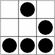
\includegraphics[width=0.5cm]{img/logo_glider.png} }
\fancyfoot[RO]{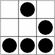
\includegraphics[width=0.5cm]{img/logo_glider.png} \hfill
	\MainTitle 
\hfill \thepage /\pageref{LastPage}}
\renewcommand{\headrulewidth}{0.25pt}
\renewcommand{\footrulewidth}{0.50pt}
\addtolength{\headheight}{0.5pt}
\fancypagestyle{plain}{
	\fancyhead{}
	\renewcommand{\headrulewidth}{0pt}
}

%--- Definitions de nouvelles commandes ---
\newcommand{\N}{\mathbb{N}} % les entiers naturels

%--- Definitions de nouvelles couleurs ---
\definecolor{verylightgrey}{rgb}{0.8,0.8,0.8}
\definecolor{verylightgray}{gray}{0.80}
\definecolor{lightgrey}{rgb}{0.6,0.6,0.6}
\definecolor{lightgray}{gray}{0.6}

%============================= Corps =================================
\begin{document}

\setlength\parindent{0pt}

%% ~\\
\vfill

\begin{center}
	\textbf{\Large \MainTitle }~\\
	~\\ ~\\ ~\\
	\texttt{http://double.co.nz/creatures/}~\\
\end{center}

\tableofcontents

\listoftables


\listoffigures

\vfill

~\\

\clearpage

%% \section{Special notes about Genetics of Creatures}

\section{Genetics} % CDR -- 

The behavior of a norn and its interaction with the environment within Creatures is controlled by its Digital DNA. This DNA code can be modified using the Creatures Genetics Kit. The Genetics Kit is the official means of editing a norns genome but there are various third party tools available as well. See the links page for other sites that may contain such utilities.~\\

While this documentation concentrates mainly on the Norn brain lobes there are a number of other genes that are modifiable via the Genetics Kit. The online help in the Genetics Kit is not very helpful when it comes to descriptions of the individual fields within each gene dialog box. Follow the links below to get information on the various fields for each gene dialog in the Genetics Kit based upon information I've gathered on the net and experiments I've performed.~\\

% 	\begin{center}
%		\begin{tabular}{p{0.6\textwidth} p{0.4\textwidth} }
\begin{minipage}{0.5\linewidth}
			\subsection{Genes}
			\begin{itemize}
				\item Brain Lobe
				\item Chemical Receptor
				\item Chemical Emitter
				\item Chemical Reaction
				\item Chemical Half-Lives
				\item Chemical Initial Concentrations
				\item Stimulus
				\item Genus
				\item Appearance
				\item Pose
				\item Gait
				\item Instinct
				\item Pigment
				\item Pigment Bleed
			\end{itemize}
\end{minipage}
			% &
\begin{minipage}{0.1\linewidth}\end{minipage}
\begin{minipage}{0.4\linewidth}
			\subsection{Reference Tables}
			\begin{itemize}
				\item State Variable Rules
				\item Cell List connection % ~\cite{genornics}
				\item Brain Map and Models % ~\cite{genornics}
			\end{itemize}
			
			\rule{3cm}{0.25mm}
			
			\rule{3cm}{0.25mm}
			
			\emph{The information presented here was written for Creatures 1 but all the information is still valid for Creatures 2 genetics. I have not yet updated the screenshots of the genetics kit for Creatures 2 but not much new was added that needs explanation.}
\end{minipage}
%			\\
%		\end{tabular}
%	\end{center}
~\\~\\
\rule{10cm}{0.5mm}

% \clearpage

\section{Brain Lobes} % CDR -- 

The brain lobe is one of the most complicated portions of norn genetics. The Cyberlife Genetics Kit provides the ability to add, delete or modify brain lobes. The dialog box for modifying brain lobes contains a bewildering number of options. The purpose of this brain lobe discussion is to describe what each of these options does.~\footnotesize{Note 08/10/1999: The information on brain lobes below was created for Creatures 1. All the information is still valid for Creatures 2 genomes, but the screen shots show the Creatures 1 genetics kit.}~\normalsize{}~\\

% \clearpage

The descriptions of the brain lobe settings shown here have mostly been discovered through experimentation. The tutorials available in another section  describes how most of the information was found. The purpose of this section is to provide a single place where all the information gathered through the tutorials and other places can be placed for easy use. It will be updated frequently as I discover new things.

\subsection{Overview}

Most standard norns have nine brains lobes. A number of the lobes are 'special' in that they have a particular function hard-coded within the Creatures executable. A limited amount of genetic modification can be done to these lobes as most of their functionality is provided through the Creatures system. The other lobes are completely genetically defined and this is where some of the most interesting modifications to a Norn can be made.~\\

\clearpage

A brain lobe sits within a 64x48 grid of neurones (often referred to here as cells). A lobe has a location within this brain grid described as an (X, Y) coordinate and (width, height). Each lobe therefore has a set size measured in neurones. Each neurone in a lobe has a numeric value associated with it known as the 'state' represented as a number from between 0 and 255 inclusive. The current value of the 'state' of a neuron indicates the level of activity. The value of the neurone 'state' can be set via the Creatures executable directly, CAOS macro code, or via dendritic links from other cells in other brain lobes. In this manner a network of cells and lobes is created that ultimately forms the 'brain' or neural net of the norn.~\\

All neurones within a single lobe behave in a similar manner to perform some function. Each lobe has genetically defined information associated with it that affects the neurones in that lobe. So a brain lobe is really a group of neurones that perform in a similar manner.~\\

%\rule{10cm}{0.5mm}~\\~\\
A detailed description of the genetically defined information associated with each lobe follows. This is the information that was obtained through experimentation. After this a brief description of the functionality of the brain lobes in a standard norn is provided. This document will conclude with some ideas and thoughts on future brain modifications that could be made to improve or modify a norns behavior.

\subsection{Brain Lobe Genetics - Genes' Header}

The Cyberlife Genetics Kit has a 'tabbed' dialog box for modifying the genetic information associated with a brain lobe. Each page of the dialog box holds information about the lobe and the breakdown below will be done page by page as defined by the genetics kit.~\\~\\~\\

\textbf{\textit{General Page}}~\\

\begin{minipage}{0.4\linewidth}
\begin{figure}[H]
	\centerline {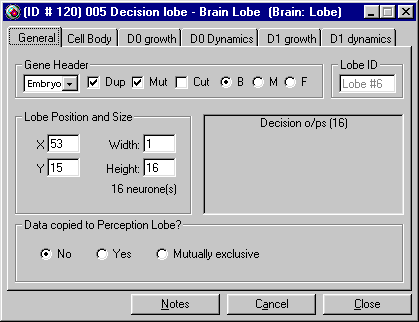
\epsfig {file=img/brain_general.png,width=5cm}} % 14.8cm
	\caption{General Interface for Brain Genetics Design}
	\label{fig:brain_general}
\end{figure}
\end{minipage}
\begin{minipage}{0.1\linewidth}\end{minipage}
\begin{minipage}{0.5\linewidth}
The example dialog given here is from the Decision lobe of a Ron norn. The 'general' page provides the standard gene header information that describes when the gene switches on, how mutations affect it and the required sex of the norn for the gene to switch on. Also included is information on the placement of the lobe within the brain grid, a description of the lobe, a unique numeric identifier for the lobe and an indication as to whether lobe data is copied to the perception lobe.
\end{minipage}~\\

\textbf{\textit{Gene Header}}
\begin{itemize}
	\item[] \emph{Embryo} : This field indicates the age at which the brain lobe gene will switch on. Most brain lobes turn on at the 'Embryo' stage to ensure they operate correctly as soon as the norn is born. I know of no lobes that are turned on at different ages and I don't know if this functionality even works. This has been added to the list of issues to explore.
	\item[] \emph{Dup} : If this flag is checked then the lobe can be duplicated as a genetic mutation. That is, multiple copies of this lobe will be able to exist due to mutation.
	\item[] \emph{Mut} : Sets whether genetic mutations can be applied to the values contained within this brain lobe.
	\item[] \emph{Cut} : If set the brain lobe can be removed during breeding or as the result of mutation. Most brain lobes have this unchecked as a norn without any of the standard lobes would not be able to function.
	\item[] \emph{B/M/F} : Defines the gender that this brain lobe will switch on. This could potentially be used to create norns that have different intelligence levels or behaviour depending on the gender of the norn. I haven't tested if this functionality actually works. This has been added to the list of issues to explore.
\end{itemize}~\\

\clearpage

\textbf{\textit{Lobe Id}}
\begin{itemize}
	\item[] \emph{Lobe \#} : Contains the numeric identifier for the brain lobe. This is assigned automatically by the genetics kit and cannot be changed. The first 8 numbers (0 through to 7) correspond to specific lobes that are hard-coded within the Creatures executable. If you number a lobe with one of these hard coded numbers (using a hex editor or such like) then Creatures may stomp over your neurone values at any time so be warned.
\end{itemize}

% \clearpage
\textbf{\textit{Lobe Position and Size}}
\begin{itemize}
	\item[] \emph{X} : Contains the X coordinate of the lobes location within the brain grid. I don't know what the effect of overlapping brain lobes will be. Added to the issues list.
	\item[] \emph{Y} : Contains the Y coordinate of the lobes location within the brain grid.
	\item[] \emph{Width} : Contains the amount of neurones in the X direction that the lobe uses within the brain grid.
	\item[] \emph{Height} : Contains the amount of neurones in the Y direction that the lobe uses within the brain grid.
\end{itemize}

The total number of neurones contained within the lobe is calculated as (Width * Height).~\\ % and displayed in the dialog box.~\\ % I do not know if the layout of the lobe or location within the brain grid has any affect on the functionality of the lobe. % Added to the issues list.

\textbf{\textit{Description}}

This contains a description of the functionality of the brain lobe and is not editable. I think only the standard brain lobes have descriptions associated with them. All additional lobes get a default like 'Interneurone lobe'.~\\

\textbf{\textit{Data Copied to Perception Lobe}}
\begin{itemize}
	\item[] \emph{No} : None of the information in this brain lobe will be duplicated in the perception lobe (lobe 0).
	\item[] \emph{Yes} : Every neurone within this brain lobe will have its state value duplicated in the perception lobe. See the perception tutorial for details.
\item[] \textit{Mutually Exclusive} : A lobe marked as mutually exclusive affects the way dendrites are formed between the perception lobe and the concept lobe. If a lobe is marked as mutually exclusive then only one cell from this lobe may contribute to the forming of a particular concept in the concept lobe. See the perception tutorial for details. 
\end{itemize}

\subsection{Cell Body Page}

\begin{minipage}{0.5\linewidth}
\begin{figure}[H]
	\centerline {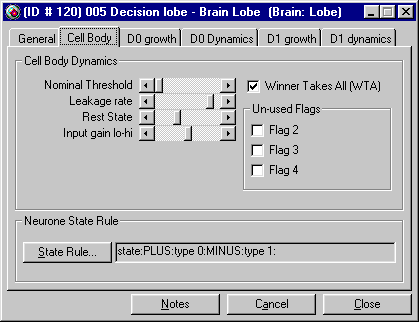
\epsfig {file=img/brain_cellbody.png,width=5cm}} % 14.8cm
	\caption{Cell Body Interface for Brain Genetics Design}
	\label{fig:brain_cellbody}
\end{figure}
\end{minipage}
\begin{minipage}{0.1\linewidth}\end{minipage}
\begin{minipage}{0.4\linewidth}
The 'Cell Body' page provides information associated with each neurone (otherwise known as 'cell') within the brain lobe. It is here that the behaviour of the neurones are defined. Much of the information obtained about this page is from tutorial one and tutorial two.
\end{minipage}~\\

% \clearpage

\textbf{\textit{Cell Body Dynamics}}
\begin{itemize}
	\item[] \emph{Nominal Threshold} : This is a number with a value from 0 through to 255. When the state is set for a neurone it will not fire unless the value of the neurone state is greater than this threshold. The value of the neurone after firing will be state minus threshold.
	\item[] \emph{Leakage Rate} : This defines the speed at which the state will drop from its current value to its rest state. It has values like 'Instantly', '5 Seconds', right through to '52 Years' and is represented by a number from 0 to 255.
	\item[] \emph{Rest State} : This is the resting state of the neurone. That is, if the neurone has not been fired or activated it will sit on the value set here. The value is from 0 through to 255.
	% \item[] \emph{Input gain lo-hi} : I have no idea what this value does. Added to issues list.
	\item[] \emph{Winner Takes All} : If this flag is checked then the lobe is a winner-takes-all lobe. This means that after all the neurone values for the lobe are calculated the highest firing neurone (highest state value) is the only one that fires and all the other neurones have their output value set to zero. An example is the decision lobe where only one decision can be made.
\end{itemize}
\clearpage
% \textbf{\textit{Un-used Flags}} : These flags do not appear to be used in any way.~\\

\textbf{\textit{Neurone State Rule}}

An SVRule is like a miniature program written in a special programming language, which has a number of 'opcodes' or operations that it can perform on various pieces of data. Only eight individual opcodes are allowed in an SVRule making it very small and fast to execute - the SVRule for every cell in the brain must execute 10 times per second! -- \emph{\underline{State Rule}} : The SVRule defined here is used to calculate the new state value of a neurone. The result of the SVRule becomes the state value of the neurone. In this way the state for neurones within lobes can be defined genetically and different calculations can be performed depending upon the task of the lobe. The SVRule possibilities are huge and can be of a great complexity. Remember that SVRules are used in a number of places in a brain lobe but the specific one here is only used to calculate the value of each neurone 'state'. % See the state variable rule page for a description of SVRules in general and what each opcode does.

\subsection{D0 Growth Page}

\begin{minipage}{0.6\linewidth}
\begin{figure}[H]
	\centerline {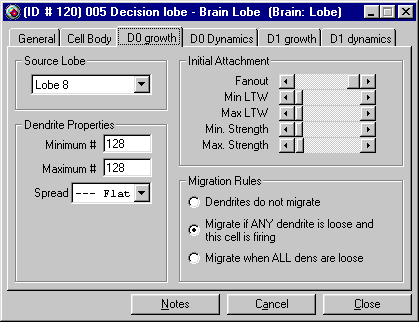
\epsfig {file=img/brain_d0growth.png,width=5cm}} % 14.8cm
	\caption{D0 growth Interface for Brain Genetics Design}
	\label{fig:brain_d0growth}
\end{figure}
\end{minipage}
\begin{minipage}{0.1\linewidth}\end{minipage}
\begin{minipage}{0.4\linewidth}
This is one of the first pages that describes the behaviour of dendrite connections in a lobe. Dendrites are to the brain lobes as wiring is to integrated circuits. They connect the neurones in different lobes and allow information to travel between them. Each brain lobe can have dendrite connections with up to two different source lobes. These are described as 'type0' dendrites and 'type1' dendrites. This page describes the settings for 'type0' dendrites.
\end{minipage}~\\~\\

% Dendrite connections are probably the most complicated part of the norn brain structure and much of what is described here is still being explored by me. If you don't understand any of what follows please email me and I'll make an effort to make it easier to understand.\\

\textbf{\textit{Source Lobe}} : This defines the brain lobe these dendrites are connected to. Data flows from neurones in the source lobe defined here to neurones in this brain lobe. ~\\ % \underline{Brain lobe construction where information comes from.}~\\ % does not define where information goes to but

\textbf{\textit{Dendrite Properties}}
\begin{itemize}
	\item[] \emph{Minimum \#} : Defines the minimum number of dendrites that will be connected between each cell in the current lobe and a source lobe cell.
	\item[] \emph{Maximum \#} : Defines the maximum number of dendrites that will be connected between each cell in the current lobe and a cell in the source. %lobe. 
	\item At birth a norn will have a random brain wiring pattern set up. Each cell will have a number of dendrites ranging between the minimum and maximum number defined here. As dendrites migrate the minimum and maximum numbers are important as they define whether there is room for a new dendrite connection to be made or removed. The decision on how many dendrites to use when creating a lobe depends upon the type of information to obtain from the source lobe and what to do with it.
	\item[] \emph{Spread} : This appears to define the pattern used to define the 'fanning' of the dendrite connection between the current lobe and the source lobe. The options are 'Flat', 'Normal', 'Saw' and 'waS'. If the spread is 'flat' then there will be two dendrites connecting neurone x from the source lobe to neurone x in the destination lobe, then (x+1) to (x+1), etc. With the other settings, a connection from neurone x in the current lobe to neurones x and (x+1) in the source lobe, from neurone (x+1) to neurones (x+1) and (x+2), etc. The exact layout of the dendrites will also depend on the 'fanout' value described later.
\end{itemize}~\\

\textbf{\textit{Initial Attachment}}
\begin{itemize}
	\item[] \emph{Fanout} : When the dendrite wiring for a brain lobe is initially created on birth of a creature, this value defines how each dendrite connection from the current lobe 'fans out' to neurones in the source lobe. The value varies from 0 through to 8.
	\item[] \emph{Min LTW} : A number ranging from 0 through to 255 described as the minimum Long Term Weight. A dendrite has a value known as the long term weight (LTW) and it has a minimum and maximum possible value. It's actual value floats somewhere in between the minimum and maximum. % The function of LTW is described in the dendrite section. These numbers are only used when initially setting the values of the dendrite upon birth. % of a norn.
	\item[] \emph{Max LTW} : The maximum value of the Long Term Weight as a number from 0 through to 255. It must be equal to or greater than the min LTW.~\\
	\item[] \emph{Min Strength} : Each dendrite has a strength value represented as a number from 0 through to 255. The strength represents how 'strong' the link between the source neurone and the current neurone. When the strength is '0' then the dendrite may migrate as the link is not strong. The minimum number defined here is used for the initial wiring of the brain lobe and for initial values after dendrite migration.
	\item[] \emph{Max Strength} : The maximum strength value that can be assigned to a dendrite on initial brain wiring.
\end{itemize}~\\

\textbf{\textit{Migration Rules}}

The radio button settings here define how dendrites will migrate between cells. An example of dendritic migration is the connections between the perception lobe and the concept lobe. The perception lobe is the source lobe and the concept lobe is the destination lobe. There may be several neurones from the source lobe connected to a single cell in the destination lobe. As a norn is punished then the connections on the source lobe neurones will migrate to other source lobe neurones to form more appropriate 'concepts' for the norn to learn and make decisions from. 
\begin{itemize}
	\item[] \emph{Dendrites do not migrate} : With this setting dendrites will not migrate at all and stay with the initial connections made at birth. This is most often used when the maximum and minimum number of dendrites is one with a flat spread. Nothing needs to migrate.
	\item[] \emph{Migrate if ANY dendrite is loose and this cell is firing} : If a neurone in the current lobe has a number of dendrites attached to a source lobe, this setting will cause the dendrites to migrate if any of these dendrites has a strength of zero and the neurone is currently firing. If a dendrite in the neurone is loose (ie. has strength of zero) but the neurone is not firing then no migration will occur. Only one of the dendrites has to be loose for the migration to occur.
	\item[] \emph{Migrate when ALL dendrites are loose} : In this case every dendrite from a given neurone in the current lobe must have a strength of zero for the dendrites to migrate. If only one is zero then no migration will occur.
\end{itemize}

% \clearpage

\subsection{D0 Dynamics Page}

\begin{minipage}{0.4\linewidth}
\begin{figure}[H]
	\centerline {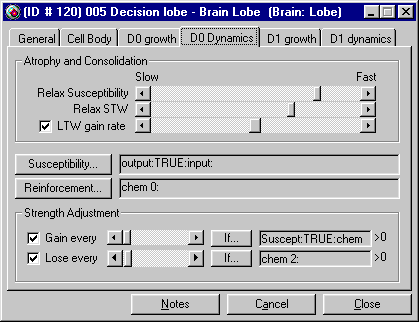
\epsfig {file=img/brain_d0dynamics.png,width=5cm}} % 14.8cm
	\caption{D0 dynamics Interface for Brain Genetics Design}
	\label{fig:brain_d0dynamics}
\end{figure}
\end{minipage}
\begin{minipage}{0.1\linewidth}\end{minipage}
\begin{minipage}{0.5\linewidth}
This is probably the most complicated portion of norn genetics. The definition of the dynamics of the dendrites. The 'D0' page describes the dynamics for the 'type0' dendrites. The dynamics defines how the strength value of a dendrite is adjusted, how the STW and LTW are adjusted, etc.~\\

A number of values are associated with a dendrite. A brief description follows to make it easier to understand what the settings on this page mean. Most of these definitions were obtained from the paper by Steve Grand \textit{et al} obtained from the Cyberlife web site.
\end{minipage}~\\

\begin{itemize}
	\item[] \emph{STW} : Short Term Weight - used to modulate input signals. STW is constantly relaxing towards LTW. It is the STW combined with the input value from the source lobe that is used to calculate the 'dendrite value'. The formula used appears to be: $dendrite value = source cell * ( stw / 255 )$~\\
where 'source cell' is the value of the cell that this dendrite is attached to from the source lobe and 'stw' is the dendrites current short term weight value. \underline{The formula for calculation of STW appears to be: } $stw = ltw + ( susceptibility / 255 ) * reinforcement$. 
	\item[] \emph{LTW} : Long Term Weight - acts as a rest state for STW and provides statistical response to reinforcement. LTW is constantly rising towards STW. LTW and STW move towards each other at different rates (and these rates are defined genetically).
	\item[] \emph{Susceptibility}: Current susceptibility to reinforcement. As can be seen in the STW calculation above, the susceptibility modulates the reinforcement value. So the higher the 'susceptibility' value, the more 'reinforcement' affects the short term weight value. 
	\item[] \emph{Strength} : Controls dendrite migration. Represents how 'strong' the dendrite link is. If strength hits zero then the link is not strong and may migrate.
\end{itemize}
\clearpage

\textbf{\textit{Atrophy and Consolidation}}
\begin{itemize}
	\item[] \emph{Relax Susceptibility} : The is the half-life of the 'susceptibility' of the dendrite. It is a value from 0 through to 255 and defines a time interval in a similar manner to that of 'Leakage Rate' in 'Cell Body Dynamics'. The value shown in the image above is 20 seconds. So when the susceptibility of a dendrite is set via the Susceptibility SVRule this setting describes how quickly it 'relaxes' back to the rest state. The relationship between this value and the susceptibility SVRule is similar to that of 'Leakage Rate' and 'State SVRule' in the 'Cell Body' page.
	\item[] \emph{Relax STW} : This is the half-life or relaxation rate of the Short Term Weight value for the dendrite. The value in the image above represents 5 minutes. Once again it is a number from 0 through to 255 representing a time span. The STW relaxes towards the Long Term Weight (LTW) value of the dendrite. This relax rate sets the speed of that relaxation.
	\item[] \emph{LTW Gain Rate} : If this option is checked then LTW constantly rises towards STW at the rate defined in the slider box. This number is a rate in the same manner as all the other leakage rates (even through the genetics kit does not display it as such). For example, if set to 10 seconds (a value of 40) then the LTW will increment by one every 10 seconds until it reaches its rest state (which is the value of STW).
	\item[] \emph{Susceptibility} : An SVRule that defines how the susceptibility to reinforcement for that dendrite. The higher the value of the result of this svrule, the more effect 'reinforcement' has on the value of STW. The SVRule defined in the image above basically says if there is an output value for the cell (ie. it is firing) then the susceptibility of the dendrite is equal to that of the input value. 
	\item[] \emph{Reinforcement} : This is the SVRule used to compute changes in STW. Typically it is set to the value of some chemical. This chemical is adjusted using the various receptors/emitters available in a norn. The STW is increased based upon the value computed by this SVRule modulated by the value of the susceptibility SVrule. In the example above it means that STW is adjusted when the amount of brain lobe chemical 0 changes in this norn.
\end{itemize}

The relationship between STW, LTW, susceptibility and reinforcement is shown by the following formulae that is used to calculate the values: 
$dendrite value = source cell * ( stw / 255 )$ and $stw = ltw + ( susceptibility / 255 ) * reinforcement$.~\\

\textbf{\textit{Strength Adjustment}}
\begin{itemize}
	\item[] \emph{Gain Every} : If this is checked then the strength value of the dendrite connection will be increased by the value indicated in the slider (from 0 through to 255) if the result of the given SVRule expression is greater than zero. The SVRule given above is 'Suscept:TRUE:chem0:TRUE:STW'. I believe that this expression means that if the susceptibility of the connection is greater than zero and chemical 0 is greater than zero then the value of the expression is STW. So the dendrite will be strengthened if it is susceptible to reinforcement, has chemical 0 and the STW is greater than zero.
	\item[] \emph{Lose Every} : If this is checked then the strength value of the dendrite connection will be decreased by the value indicated in the slider (from 0 through to 255) if the result of the given SVRule expression is greater than zero. The SVRule given above is 'chem 2'. So if the value of chemical 2 is greater than zero then the strength of the dendrite will be reduced.
\end{itemize}

\subsection{Dendrite Overview}

This is a brief outline of how dendrite values are calculated mostly obtained from the technical papers available at the cyberlife web site. I'll add to this and hopefully provide some programs that demonstrate how things work to make it easier to understand. The following is quoted from one of the technical papers by Steve Grand \textit{et al}:~\\

% \clearpage

\emph{After disturbance, both the STW and the LTW relax exponentially towards other, with the LTW being the slower. The STW therefore reacts strongly to individual reinforcement episodes, while the LTW effectively computes a moving average of many STW disturbances: if a creature meets with situation X and finds that its chosen course of action was undesirable, then it should immediately be strongly disinclined to repeat the action, especially as many of the incentives to do so may still be present. However, situation X may not always be as bad as first experience suggests, and so the creatures long-term interpretation should be less sweeping}~\\

\clearpage

\emph{Dendritic Migration. The initial wiring is defined at birth according to a small number of genetic rules. Generally, neurones attempt to connect from one lobe to another in a direct spatial mapping, with multiple dendrites fanning out in a specified distribution to either side of the optimum source cell. After birth, however, individual dendrites may migrate and form new connections (always within the same source lobe). Periodically, a Strength value change is computed for each synapse using SVRules, often in response to chemical changes. If the Strength falls to zero, the dendrite disconnects and follows the appropriate rule about how to find a new connection. These migration rules were chosen in order to fulfill the requirements for the initial brain model.}

\subsection{Issues}

The following is a list of issues to be examined as I explore the functionality of each field in the genetic structure of the brain lobe gene. If you know the answer to any of these issues please email me. Meanwhile I'll be working my way through them in no particular order.
\begin{enumerate}
	%% \setlength{\itemsep}{0pt} %% useful if babel is on english...
	%% \setlength{\parskip}{0cm} %% useful if babel is on english...
	\item Can brain lobes be switched on or off based upon the gene header details. That is, can different lobes be created for different genders and can lobes be turned on when a norn hits certain ages. Is there any useful benefit that can be explored if this functionality exists.
	\item What is the effect of overlapping brain lobes? If the (X, Y, W, H) values of a lobe cause a portion to overlap another lobe what affect does this have on the values of the neurones?
	\item Does the location of a brain lobe within the brain grid or the different height and width combinations have any affect on the functionality of a brain lobe? Does it affect dendrite fanout and migration for example.
	\item What does 'Mutually Exclusive' in the 'Data Copied to Perception Lobe' do?
	\item What is the effect of changing 'input gain hi-lo' on the 'Cell Body' page?
	\item Work out the exact affect of 'spread' and fanout in the dendrite pages. Draw a diagram showing what it does instead of that horrible textual description!!
	\item Determine if the 'shape' (W, H) of a lobe affects the fanout of the dendrites.
	\item Describe the functionality of STW and LTW of dendrites.
	\item Are the Min LTW,Max LTW, Strength, etc only used for randomly setting values of the dendrites at birth? Or do they define the minimum and maximums that can apply throughout the lifetime of the dendrite?
	\item Work out exactly what each setting for the migration rules of the dendrites means.
	\item Does migration of dendrites only occur when the cell is firing in all cases?
	\item Investigate and describe what all the values for a dendrite are (susceptibility, etc).
	\item Investigate how susceptibility works.
	\item Document what time span each number in the half-life sliders relates to.
	\item Write a program that demonstrates how STW, LTW, etc interact.
	\item Expand and refine the dendrite overview.
\end{enumerate} %% ~\\

\textbf{Progress on Issues}%% ~\\

\textbf{Issue 3}%% ~\\

	Yes the height and width of a lobe affects the original dendrite connections. The following image shows a source lobe of height 1, width 3 connected to a destination lobe with height 1, width 3: \emph{see figure~\ref{fig:dendrite0}}.~\\
	
	Notice how the dendrite links are basically cell by cell. Cell 0 is connected to cell 0 and1. Cell 1 is connected to cell 1 and 2, etc. If the lobes are done as a 3x3 square we get more of a spread in the connections: \emph{see figure~\ref{fig:dendrite1}}. ~\\
	
	I've only filled in a few lines here. I really need a 3D diagram to do it justice! Image the two lobes overlay each other. Now each cell can connect to the cells to either side of it. So cell 5 in the output lobe is next to cell 5 and cell 7 in the input lobe so they can be connected. Cell 8 is next to Cell 4 so it can be connected, etc. ~\\
	
	By changing the width and height of the input and output lobe you can adjust the initial spread of the dendrites - perhaps giving a wider spread than would otherwise have been done if it was one straight lobe. I believe it would also give more cell choices for dendrite migration as well. ~\\

\begin{minipage}[h]{6.00cm}
	\begin{figure}[H]
		\centerline {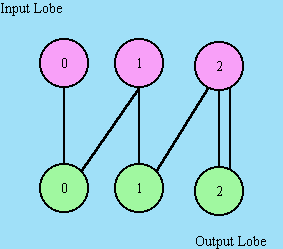
\epsfig {file=img/dendrite0.png,width=5.00cm}}
		\caption{Impact of original height and with on original connections. }
		\label{fig:dendrite0}
	\end{figure}
\end{minipage} \hfill \begin{minipage}[h]{13.50cm}
	\begin{figure}[H]
		\centerline {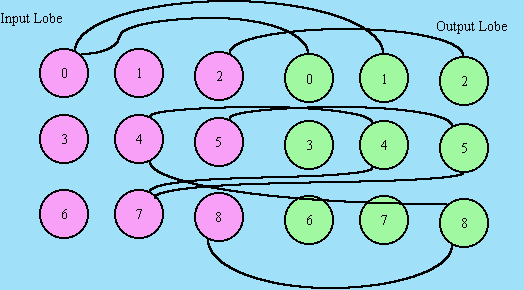
\epsfig {file=img/dendrite1.png,width=10.00cm}}
		\caption{Proximity connection of cells. }
		\label{fig:dendrite1}
	\end{figure}
\end{minipage} %% ~\\

\textbf{Issue 4} %% ~\\

Solved thanks to some pointers from a couple of anonymous tipsters. Information has been updated on the Brain Lobe page and the Perception Lobe Tutorial. %% ~\\

\subsection{Perception Lobe Tutorial}

The perception lobe works slightly differently to the other brain lobes so I've created this tutorial to demonstrate what makes it special. --- The purpose of the perception lobe appears to be to summarise everything that a norn can 'perceive' into one brain lobe so the norn can eventually store concepts and memories based upon these perceptions (done in the concept lobe). This tutorial attempts to answer the questions about how the perceptible lobes are summarised into the perception lobe and how to work out what each cell of the perception lobe means. --- The usual method of passing cell information from one lobe to another is through wiring up dendrites. Using dendrites you can only summarise information from two other brain lobes (the D0 and D1 dendrite connections). With the perception lobe there is more than two lobes that need to be summarised so it appears a mechanism specifically for dealing with the perception lobe was built. -- In the Genetics Kit each brain lobe has an option that can be set indicating whether or not the lobes data is copied to the perception lobe.

\begin{minipage}[h]{9.75cm}
	\begin{figure}[H]
		\centerline {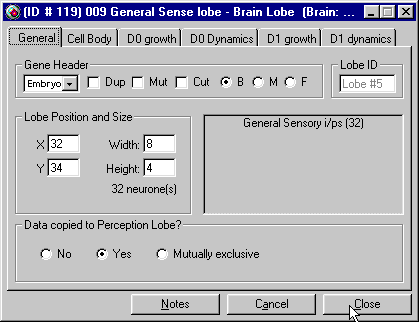
\epsfig {file=img/gensense.png,width=9.50cm}}
		\caption{General Senses. }
		\label{fig:gensense}
	\end{figure}
\end{minipage} \hfill \begin{minipage}[h]{9.50cm}
	As can been seen from the above dialog box \emph{(figure~\ref{fig:gensense})} from the general sense lobe the options for perception are:
	\begin{itemize}
		\item No
		\item Yes
		\item Mutually exclusive
	\end{itemize} ~\\
	
	The brain lobes that are marked as 'Yes' or 'Mutually exclusive' in an original norn are: ~\\
	\begin{tabular}[h]{|p{3.25cm}|p{0.75cm}|p{4.00cm}|}
		\hline
		\textbf{Lobe}		& 	\textbf{Size}	& 	\textbf{Data copied to \newline perception lobe?}	\\ \hline
		Drive lobe			&	16				&	Mutually exclusive									\\ \hline
		Verb lobe			&	16				&	Mutually exclusive									\\ \hline
		General sense lobe	&	32				&	Yes													\\ \hline
		Attention lobe		&	40				&	Yes													\\ \hline
	\end{tabular}
\end{minipage} ~\\

The perception lobe must have a number of cells equal to or greater than the total number of cells in all lobes marked as 'Yes' or 'Mutually exclusive'. The total number of cells in the above lobes equals 104. The size of the perception lobe is 112 so there is a little room to spare there. ~\\

\begin{minipage}[h]{9.00cm}
	My theory from observation is that starting from the lowest numbered perceptible lobe, the output of each cell of that lobe is copied to the lowest available cell in the perception lobe. So with the perceptible lobes listed above I think the mapping to the perception lobe cells will be: ~\\
\end{minipage} \hfill \begin{minipage}[h]{9.65cm}
	\begin{tabular}[h]{|p{4.75cm}|p{4.50cm}|}
		\hline
		\textbf{Perception cell number}	&	\textbf{Other lobe cell number}	\\ \hline
		0-15							&	Drive lobe 0-15					\\ \hline
		16-31							&	Verb lobe 0-15					\\ \hline
		32-63							&	General sense lobe 0-31			\\ \hline
		64-103							&	Attention lobe 0-39				\\ \hline
	\end{tabular}
\end{minipage} ~\\

I do not know what the setting 'Mutually exclusive' means. From my tests it appears to do the same as 'Yes' but further experimentation may show otherwise. The following examples will attempt to demonstrate whether my theory about how the perception lobe works and is mapped is correct or not. ~\\

\begin{minipage}[h]{9.00cm}
	For this example we start with a norn with the normal nine lobes selected in Creatures and we will test the lobes with Perceptible marked as 'Yes'. Run the BrainCellMonitor program, connect to Creatures, and use the 'Add' button to view the following Lobe/Cell/Dendrites:
	\begin{itemize}
		\item Lobe 0 Cell 32 Dendrite 0
		\item Lobe 0 Cell 63 Dendrite 0
		\item Lobe 5 Cell 0 Dendrite 0
		\item Lobe 5 Cell 31 Dendrite 0
	\end{itemize} ~\\
	
	This will allow us to view the first and last cell in the general sense lobe and compare it against the perceptible cell we think they will be copied to. ~\\
	
	We will now use CAOS commands to fire particular cells in the general sense lobe (lobe 5) and see if the corresponding cell in the perception lobe (lobe 0) fires with equivalent values. ~\\
\end{minipage} \hfill \begin{minipage}[h]{9.75cm}
	\begin{figure}[H]
		\centerline {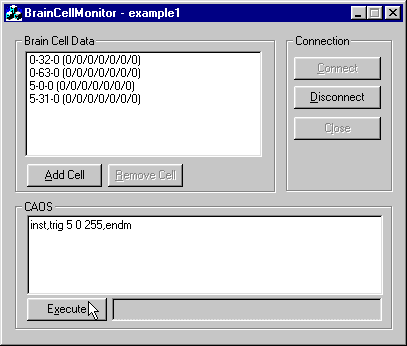
\epsfig {file=img/example1.png,width=9.50cm}}
		\caption{Brain Cell Monitor --- Example 1. }
		\label{fig:perceptionLobeExample1}
	\end{figure}
\end{minipage} ~\\

Try executing the CAOS command: \texttt{inst,trig 5 0 255,endm} --- Notice how the perception lobe cell number 32 output number increases and starts to decrease in a similar way to the general sense lobe cell we just fired: ~\\

\begin{minipage}[h]{9.75cm}
	\begin{figure}[H]
		\centerline {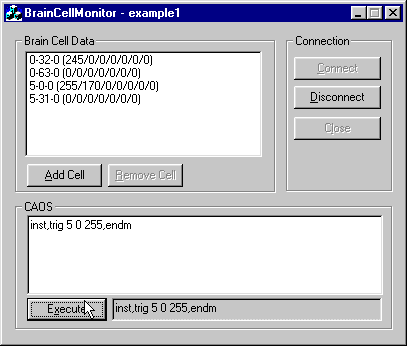
\epsfig {file=img/example2.png,width=9.50cm}}
		\caption{Brain Cell Monitor --- Example 2. }
		\label{fig:perceptionLobeExample2}
	\end{figure}
\end{minipage} \hfill \begin{minipage}[h]{9.00cm}
	This seems to imply that our assumed mapping may be correct. ~\\
	
	Try executing the CAOS command: \texttt{inst,trig 5 31 255,endm} ~\\
	
	Notice how the perception lobe cell number 63 output number increases and starts to decrease in a similar way to the general sense lobe cell we just fired. This also seems to confirm our mapping. Try using different cell numbers with lobe 5 and you will see that the mapping we came up with is correct. Now we'll try it with the Attention lobe. Use BrainCellMonitor to view the following cells: %% ~\\
	\begin{itemize}
		\item Lobe 0 Cell 64 Dendrite 0
		\item Lobe 0 Cell 103 Dendrite 0
		\item Lobe 7 Cell 0 Dendrite 0
		\item Lobe 7 Cell 39 Dendrite 0
	\end{itemize} ~\\
\end{minipage} ~\\ 

Try executing the CAOS command: \texttt{inst,trig 7 0 255,endm} and executing the CAOS command: \texttt{inst,trig 7 39 255,endm} --- Once again you should see the equivalent perception lobes firing. ~\\

You may notice that when doing the General sense example that if you fire both general sense lobes then both perception lobes also fire. But in the Attention example, firing both will only cause one perception lobe cell to fire - why is this? It is because the Attention lobe is marked 'Winner takes all'. This means that only the cell with the highest output actually fires - all the others get automatically set to zero and this data is copied to the perception lobe. ~\\

Well what about the 'Mutually Exclusive' option? Lets try some examples with the Verb lobe which is marked "mutually exclusive". I don't use the Drive lobe just yet as the drives for a norn are constantly changing and can get in the way of our observations. Try viewing the following: %% ~\\
\begin{itemize}
	\item Lobe 0 Cell 16 Dendrite 0
	\item Lobe 0 Cell 31 Dendrite 0
	\item Lobe 3 Cell 0 Dendrite 0
	\item Lobe 3 Cell 15 Dendrite 0
\end{itemize} ~\\

Try executing the CAOS command: \texttt{inst,trig 3 0 255,endm} and executing the CAOS command: \texttt{inst,trig 3 15 255,endm} --- Once again you should see the equivalent perception lobes firing. The verb lobe is also marked 'Winner takes all' so you'll see similar effects to that shown in the Attention lobe. --- You can try examples with the drive lobe as well but as mentioned before the norn drives can get in the way of observation. ~\\

The Mutually Exclusive option works in the same manner as lobes marked as 'Yes'. The difference between the two options appears when dendrites are linked between the perception lobe and the concept lobe. Usually from 1 to 3 perception cells are linked to a particular concept cell. The perception cells that are linked can change during the lifetime of a norn based on experiences it has encountered. But only one cell from a given Mutually Exclusive lobe can contribute to the forming of a particular concept. Drive is mutually exclusive so we can have a concept of 'hungry' but not 'hungry' and 'tired'. Verb lobe is also mutually exclusive so we can have a concept of being told to 'push' but not being told to 'push' and 'pull'. ~\\

%% I hope this tutorial/discussion was useful to you in examining the Perception lobe. If you come up with any interesting information I'd love to hear from you. I've updated the BrainActivity program to display the cell details in the perception lobe based on the above observations (as of version 1.3).

%% If you've been following this please send feedback to Chris Double [chris@double.co.nz] and let me know what you'd like to see. Thanks!


% \rule{10cm}{0.5mm}~\\

\clearpage

\section{Chemical Emitter} % CDR -- 

\subsection{Overview}

A chemical emitter gene controls the injection of a particular chemical into the norn based upon data retrieved from some Organ, Tissue or Locus within the norn. The Organ, Tissue or Locus is a data value controlled by the Creatures executable ranging in value from 0 through to 255. It can represent a brain cell, external stimuli or other things selected from the dialog box. Every given time period the Organ, Tissue or Locus is examined and compared against a number of settings defined in this gene. Depending upon the results of this comparison an amount of chemical can be injected into the norn.~\\

% \clearpage

\begin{minipage}{0.5\linewidth}
\subsection{Dialog Box}
\begin{figure}[H]
	\centerline {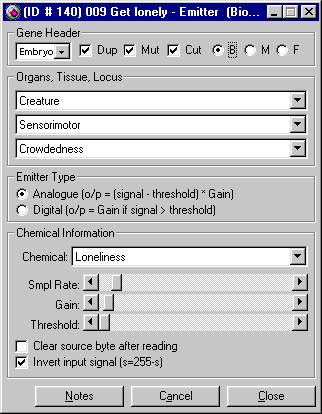
\epsfig {file=img/chemical_emitter.png,width=5.20cm}} % 11.35cm
	\caption{Interface for Chemical Emitter Design}
	\label{fig:chemical_emitter}
\end{figure}
\subsection{Breakdown -- \emph{Gene Header}}
\end{minipage}
\begin{minipage}{0.1\linewidth}\end{minipage}
\begin{minipage}{0.45\linewidth}
% \clearpage
\textbf{\textit{Gene Header}}~\\
\begin{itemize}
	\item[] \emph{Embryo} : This field indicates the age at which this gene will switch on. Most genes turn on at the 'Embryo' stage to ensure they operate correctly as soon as the norn is born. 
	\item[] \emph{Dup} : If this flag is checked then the gene can be duplicated as a genetic mutation. That is, multiple copies of this gene will be able to exist due to mutation.
	\item[] \emph{Mut} : Sets whether genetic mutations can be applied to the values contained within this gene.
	\item[] \emph{Cut} : If set the gene can be removed during breeding or as the result of mutation. 
	\item[] \emph{B/M/F} : Defines the gender that this gene will switch on. This is often used to select between genes that involve male or female functionality (eg. hormones).
\end{itemize}
\end{minipage}~\\~\\

% \textbf{\textit{Organs, Tissue, Locus}}~\\

% Defines the area of the norn that will be examined to calculate how much (if any) chemical to inject into the norn. Each of the options is represented by a data value ranging from 0 through to 255. The following table describes each possible option.~\\

%% %% http://www.ukonline.be/programmation/latex/tutoriel/chapitre13/page4.php %% table, rotate, longtable
%		\begin{longtable}{|p{0.15\textwidth}|p{0.20\textwidth}|p{0.65\textwidth}|}
%		\hline \rowcolor[gray]{0.50} \multicolumn{3}{|c|}{Organs, tissues, locus informations and description for Emitters} \\
%		\hline \rowcolor[gray]{0.75} \textbf{Box 1} & \textbf{Box 2} & \textbf{Box 3} \\ \hline
%		\endfirsthead
%		\hline \rowcolor[gray]{0.50} \multicolumn{3}{|c|}{Organs, tissues, locus informations and description for Emitters} \\
%		\hline \rowcolor[gray]{0.75} \textbf{Box 1} & \textbf{Box 2} & \textbf{Box 3} \\ \hline
%		\endhead
%		\hline 
%		\endfoot
%
%		Brain & Any Brain Lobe & \textbf{Lobe Activity} \\
%		\cline{3-3} % \hline
%				&	& \emph{Still to be investigated.} \\
%		\cline{3-3} % \hline
%				&	& \textbf{\# Loose Dens/Cells type 0} \\
%		\cline{3-3} % \hline
%				&	& \emph{Still to be investigated.} \\
%		\cline{3-3} % \hline
%				&	& \textbf{\# Loose Dens/Cells type 1} \\
%		\cline{3-3} % \hline
%				&	& \emph{Still to be investigated.} \\
%		\cline{3-3} % \hline
%				&	& \textbf{Cell(n) Output} \\
%		\cline{3-3} % \hline
%				&	& Represents the output value of the given cell in the brain lobe. See the brain lobe page for details on brain cells. \\
%		\hline \hline
%			Creature	&	Somatic	&	\textbf{Muscle Energy Used} \\
%		\cline{3-3} % \hline
%				&	& \emph{Still to be investigated.} \\
%		\cline{2-3} % \hline
%				&	Circulatory	& \textbf{Floating recip-emit n} \\
%		\cline{3-3} % \hline
%				&	& A floating recip--emit is a place that a receptor can use for storing a data value from 0--255 which an emitter can then use for any purpose. It's a means of linking a receptor directly to an emitter without going through a brain lobe. There are up to eight of these numbered from 0--7 (the 'n'). The life kit norns use this for the hunger/glycogen equation. \\
%		\cline{2-3} % \hline
%				&	Reproductive	& \textbf{I am fertile (egg/sperm ready)} \\
%		\cline{3-3} % \hline
%				&	& This will be a value of 0 until the norn becomes fertile in which case it will be 255. \emph{(Not confirmed, to be investigated).} \\
%		\cline{3-3} % \hline
%				&	& \textbf{I am pregnant (egg\&sperm ready)} \\
%		\cline{3-3} % \hline
%				&	& This will be a value of 0 until the norn becomes pregnant in which case it will be 255. \emph{(Not confirmed, to be investigated).} \\
%		\cline{2-3} % \hline
%				&	Immune	& \textbf{I'm dead (post mortem chemistry)} \\
%		\cline{3-3} % \hline
%				&	& This will be a value of 0 while the norn is alive. When the norn dies it will be 255. \emph{(Not confirmed, to be investigated).} \\
%		\cline{2-3} % \hline
%				&	Sensorimotor	& \textbf{Permanently Active (255)} \\
%		\cline{3-3} % \hline
%				&	& Always produces a value of 255. \emph{(Not confirmed, to be investigated).} \\
%		\cline{3-3} % \hline
%				&	& \textbf{I'm Asleep (255)} \\
%		\cline{3-3} % \hline
%				&	& This will be a value of 0 while the norn is awake. When the norn sleeps it will be 255. \emph{(Not confirmed, to be investigated).} \\
%		\cline{3-3} % \hline
%				&	& \textbf{Air is this cold} \\
%		\cline{3-3} % \hline
%				&	& This is always zero. It is not connected in Creatures 1. \\
%		\cline{3-3} % \hline
%				&	& \textbf{Air is this hot} \\
%		\cline{3-3} % \hline
%				&	& This is always zero. It is not connected in Creatures 1. \\
%		\cline{3-3} % \hline
%				&	& \textbf{Light level} \\
%		\cline{3-3} % \hline
%				&	& A value from 0--255 indicating the light level. \emph{(Not confirmed, to be investigated).} \\
%		\cline{3-3} % \hline
%				&	& \textbf{Crowdedness} \\
%		\cline{3-3} % \hline
%				&	& A value from 0--255 indicating the current crowdedness of the norn. \emph{(Not confirmed, to be investigated).} \\
%		\cline{2-3} % \hline
%				&	Drive Levels	& \textbf{Drive Lobe} \\
%		\cline{3-3} % \hline
%				&	& The current value of the given drive represented as a number from 0--255. \\
%		\hline
%	\caption{Organs, tissues, locus informations and description for Emitters}
%	\label{tab:Emitter_OrganTissuesLocus}\\
%	\end{longtable}

\textbf{\textit{Emitter Type}}
\begin{itemize}
	\item[] \emph{Analogue} : The amount of chemical injected into the norn will be proportional to the signal level received from the locus. The following formula will be applied to know how much chemical to inject: $(signal - threshold) * (gain / 255)$.
	\item[] \emph{Digital} : A constant amount ('gain') of chemical will be injected into the norn when the 'signal' reaches a specified 'threshold'. 
\end{itemize}~\\

\textbf{\textit{Chemical Information}}
\begin{itemize}
	\item[] \emph{Chemical} : Defines the chemical that will be added to the norn.
	\item[] \emph{Smpl Rate} : Sample Rate (inverted) indicates how often the emitter is processed and therefore how often the chemical will be injected. % The higher the value the slower the rate. A rate of zero is instantaneous and a rate of 255 appears to be almost never.
	\item[] \emph{Gain} : Defines how much chemical will be injected. Note that this will increase the amount of chemical into by the given amount, not replace it. See the description of 'Emitter Type' above for the calculation used~\\
	\item[] \emph{Threshold} : The locus must be firing at this level for a chemical injection to occur. In the case of Digital emitters the signal from the locus must be greater than this threshold. For Analogue emitters the signal is reduced by the amount of this threshold. See 'Emitter Type' above for the calculation. 
	\item[] \emph{Clear Source Byte after Reading} : After the emitter is processed the locus value will be reset to zero if this option is selected.
	\item[] \textit{Invert Input Signal} : The signal value used in all calculations in the emitter will be $255-signal$ if this option is selected. This new signal value will then be used for all emitter calculations (including against the threshold).
\end{itemize}

% \clearpage

\section{Chemical Receptor} % CDR -- 

\begin{minipage}{0.5\linewidth}
\subsection{Overview}
A chemical receptor gene allows an Organ, Tissue or Locus within the norn to be changed based upon the level of a chemical within that norn. The chemical associated with the receptor is constantly monitored to see if it surpasses a given threshold. When that threshold is reached a formula is calculated from the chemical amount and the result is applied to the Organ, Tissue or Locus selected.
\end{minipage}
\begin{minipage}{0.1\linewidth}\end{minipage}
\begin{minipage}{0.5\linewidth}
\subsection{Dialog Box}
\begin{figure}[H]
	\centerline {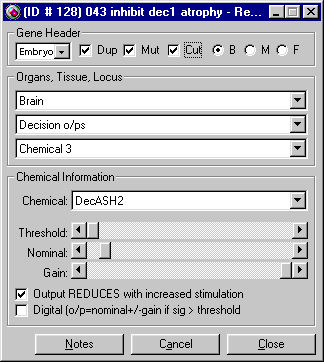
\epsfig {file=img/chemical_receptor.png,width=5.20cm}} % 11.43cm
	\caption{Interface for Chemical Receptor Design}
	\label{fig:chemical_receptor}
\end{figure}
\end{minipage}

\subsection{Breakdown}

\textbf{\textit{Gene Header}} : \emph{The gene header is the same for all genes. }~\\

% \textbf{\textit{Organs, Tissue, Locus}}~\\

% Defines the area of the norn that will have the result of the receptor formula applied to it. The result applied is a numeric value ranging from 0 through to 255 and its effect is different for each Locus. The following table describes what I believe to be the effects of each individual locus.~\\

%		\begin{longtable}{|p{0.15\textwidth}|p{0.20\textwidth}|p{0.65\textwidth}|}
%		\hline \rowcolor[gray]{0.50} \multicolumn{3}{|c|}{Organs, tissues, locus informations and description for Receptors} \\
%		\hline \rowcolor[gray]{0.75} \textbf{Box 1} & \textbf{Box 2} & \textbf{Box 3} \\ \hline
%		\endfirsthead
%		\hline \rowcolor[gray]{0.50} \multicolumn{3}{|c|}{Organs, tissues, locus informations and description for Receptors} \\
%		\hline \rowcolor[gray]{0.75} \textbf{Box 1} & \textbf{Box 2} & \textbf{Box 3} \\ \hline
%		\endhead
%		\hline 
%		\endfoot
%		
%			Brain & Any Brain Lobe & \textbf{Threshold} \\
%		\cline{3-3} % \hline
%				&	& Still to be investigated. If it allows adjustment to the threshold value of the given brain cell then it opens up a number of possibilities in brain modifications. The threshold is usually statically defined in the brain lobe gene - allowing it to be updated dynamically in this manner could be interesting. \\
%		\cline{3-3} % \hline
%				&	& \textbf{Leakage} \\
%		\cline{3-3} % \hline
%				&	& Still to be investigated. See the threshold comment above. \\
%		\cline{3-3} % \hline
%				&	& \textbf{Gain} \\
%		\cline{3-3} % \hline
%				&	& \emph{Still to be investigated.} \\
%		\cline{3-3} % \hline
%				&	& \textbf{Den(x) relax susceptibility} \\
%		\cline{3-3} % \hline
%				&	& \emph{Still to be investigated.} The 'x' represents the dendrite type (0 or 1). See the brain lobe section for details on dendrite types. \\
%		\cline{3-3} % \hline
%				&	& \textbf{Den(x) relax STW} \\
%		\cline{3-3} % \hline
%				&	& \emph{Still to be investigated.} \\
%		\cline{3-3} % \hline
%				&	& \textbf{Den(x) relax LTW} \\
%		\cline{3-3} % \hline
%				&	& \emph{Still to be investigated.} \\
%		\cline{3-3} % \hline
%				&	& \textbf{Den(x) strength gain rate} \\
%		\cline{3-3} % \hline
%				&	& \emph{Still to be investigated.} \\
%		\cline{3-3} % \hline
%				&	& \textbf{Den(x) strength loss rate} \\
%		\cline{3-3} % \hline
%				&	& \emph{Still to be investigated.} I believe all these Den(x) parameters allow dynamic changing of the various options available in the dendrite sections of the brain lobes. This could allow some interesting modifications to learning and reinforcement based upon external factors to the norn.\\
%		\cline{3-3} % \hline
%				&	& \textbf{Chemical n} \\
%		\cline{3-3} % \hline
%				&	& Where 'n' is a value from 0 to 3. Still to be investigated but like the above I believe it will change the amount of the particular brain chemical for the given lobe. \\
%		\cline{3-3} % \hline
%				&	& \textbf{Cell(n) State} \\
%		\cline{3-3} % \hline
%				&	& Represents the state value of the given cell in the brain lobe. See the brain lobe page for details on brain cells. \\
%
%		\hline \hline
%			Creature	&	Somatic	& \textbf{Become a child} \\
%		\cline{3-3} % \hline
%				&	& Changes the life stage of the norn to that of 'child'. The current norn genome sets this at a default value until aging chemical hits a certain level then it will drop to zero. From this I assume that a zero value indicates it has reached this particular life stage. To be investigated further. \\
%		\cline{3-3} % \hline
%				&	& \textbf{Become adolescent} \\
%		\cline{3-3} % \hline
%				&	& \emph{See above.} \\
%		\cline{3-3} % \hline
%				&	& \textbf{Become youth} \\
%		\cline{3-3} % \hline
%				&	& \emph{See above.} \\
%		\cline{3-3} % \hline
%				&	& \textbf{Become old} \\
%		\cline{3-3} % \hline
%				&	& \emph{See above.} \\
%		\cline{3-3} % \hline
%				&	& \textbf{Become senile} \\
%		\cline{3-3} % \hline
%				&	& \emph{See above.} \\
%		\cline{3-3} % \hline
%				&	& \textbf{Die of old age} \\
%		\cline{3-3} % \hline
%				&	& \emph{See above.} \\
%		\cline{3-3} % \hline
%				&	& \textbf{Become adolescent} \\
%		\cline{3-3} % \hline
%				&	& \emph{See above.} \\
%		\cline{2-3} % \hline
%				&	Circulatory	& \textbf{Floating recip-emit n} \\
%		\cline{3-3} % \hline
%				&	& A floating recip-emit is a place that a receptor can use for storing a data value from 0-255 which an emitter can then use for any purpose. It's a means of linking a receptor directly to an emitter without going through a brain lobe. There are up to eight of these numbered from 0-7 (the 'n'). The life kit norns use this for the hunger/glycogen equation. See the notes section at the end of this page for a description of this mechanism. \\
%		\cline{2-3} % \hline
%				&	Reproductive	& \textbf{Become fertile if high} \\
%		\cline{3-3} % \hline
%				&	& In the C1 genome this tracks the Oestrogen or Testosterone (Females and Males respectively) chemical exactly. To be investigated (but probably means the obvious). \\
%		\cline{3-3} % \hline
%				&	& \textbf{Receptive to sperm if >0} \\
%		\cline{3-3} % \hline
%				&	& If greater than zero then the norn is receptive to sperm. In the C1 genome it is linked to sex drive for females. From what I understand this is always greater than zero as a result of the receptor in the C1 genome. \emph{To be investigated.} \\
%		\cline{2-3} % \hline
%				&	Immune	& \textbf{Die if non-zero} \\
%		\cline{3-3} % \hline
%				&	& If the value of this is ever non-zero the norn will die. In the various life kit genomes it is linked to the aging chemical. When the chemical is lower than a certain value the norn will die. \\
%		\cline{2-3} % \hline
%				&	Sensorimotor	& \textbf{Involuntary Action n} \\
%		\cline{3-3} % \hline
%				&	& Where 'n' is a number from 0 through to 7. Activates the particular involuntary action. \emph{To be investigated.} \\
%		\cline{3-3} % \hline
%				&	& \textbf{<normal walk gait (do not use)>} \\
%		\cline{3-3} % \hline
%				&	&  \emph{To be investigated.} \\ 
%		\cline{3-3} % \hline
%				&	& \textbf{Special gait n} \\
%		\cline{3-3} % \hline
%				&	&  Where 'n' is a number from 1 through to 7. \emph{To be investigated.} \\
%		\cline{2-3} % \hline
%				&	Drive Levels	& \textbf{Drive Lobe} \\
%		\cline{3-3} % \hline
%				&	& Allows setting of the drive level for a norn. In the C1 genome this is set to match the particular drive chemical exactly. \\
%		\hline
%	\caption{Organs, tissues, locus informations and description for Receptors}
%	\label{tab:Receptor_OrganTissuesLocus}\\
%	\end{longtable}

\textbf{\textit{Chemical Information}}
\begin{itemize}
	\item[] \emph{Chemical} : Defines the particular chemical that will be monitored. %  by the receptor
	\item[] \emph{Threshold} : Defines the level of the chemical that must exist before the given locus is activated. In the case of Digital receptors the amount of chemical must be greater than this threshold before the locus is activated. For Analogue receptors the signal (ie. amount of chemical) is reduced by the amount of this threshold before calculating the amount to stimulate the locus by. See Formula below for the calculation used.
	\item[] \emph{Nominal} : Defines the default or base value used to stimulate the locus. This what the locus will be set to if the amount of chemical is not greater than the threshold. 
	\item[] \emph{Gain} : Defines what the value of the locus will be set to in the case of a digital receptor or as a scaling factor for calculating the amount in an analog receptor. See Formula below for details.
	\item[] \emph{Output REDUCES with increased stimulation} : If this is checked then all adjustments to the base value of the receptor (ie. the Nominal amount) will reduce that base value. If cleared all adjustments will increase the base value.
	\item[] \emph{Digital} : The locus will be set to a constant amount if the chemical amount is greater than a certain threshold if this option is checked. If it is unchecked then the receptor is analogue. This means that the locus will be set to a value in proportion to the amount of chemical. See below for details.
\end{itemize}

\textbf{\textit{Formula}}

\underline{Analogue receptors} formula for calculating the value for the locus:

$Nominal + (((ChemicalAmount - Threshold) * Gain/255) * R)$

Where R is 1 if 'Output Reduces with increased stimulation' is not checked and -1 if it is checked. So the nominal will be reduced or increased based upon this flag.~\\

\underline{Digital receptors} formula for calculating the value for the locus:

$Nominal + ((ChemicalAmount > Threshold ? Gain : 0) * R)$

So if the chemical amount is greater than the threshold then the locus setting will be the Nominal amount increased or decreased by the Gain depending on the setting of 'R'. If it is not greater than the threshold then the locus setting will be equivalent to Nominal.~\\

% \subsection{Notes}
% I've found that the norn genome has become much clearer to me now that I understand exactly how the receptor is calculated. And the possibility of dynamically modifying the various settings of the brain lobes leads to some interesting areas as well.~\\
% Using the information above I examined how the new hunger/glycogen reaction works in the life kit norns. Using a receptor the glycogen chemical is attached to floating recep-emitter number 2 (FRE-2). The settings for this emitter make FRE-2 exactly equal to the amount of glycogen chemical. So a value of 100 glycogen will cause a value of 100 FRE-2.~\\
% The hunger emitter gets it's input from FRE-2. It is an analogue emitter with a sample rate of 5, a gain of 2, a threshold of zero and it is inverted.~\\
% This means that approximately every half second or so the hunger chemical is increased by an amount equal to:~\\
% $(255 - GlycogenAmount) * 2/255$~\\
% So high glycogen means that hunger will not be increased. Glycogen has to be lower than about 100 before hunger is adjusted to any great degree. So if you don't want your norns to be hungry, keep their glycogen levels high.~\\

%%%%%%%%%%%%%%%%%%%%%%%%%%%%%%%%%%%%%%%%%%%%%%%%%%%%%%%%%%%%%%%
% % % % % % demi-vie
% \section{CDR -- Chemical Half-Life}

% \begin{minipage}{0.5\linewidth}
% \subsection{Overview}
% The chemical half-life gene defines the decay rate of all the chemicals inside a norn. Each chemical has a value ranging from 0 through to 255 representing the amount of substance within the norn. The higher the number the more chemical inside the norn.~\\
% To prevent the chemical from staying permanently within the norn you can set a decay rate. This sets a period of time over which the chemical amount will slowly drop down towards zero.
% \end{minipage}
% \begin{minipage}{0.1\linewidth}\end{minipage}
% \begin{minipage}{0.4\linewidth}
% \subsection{Dialog Box}
% \begin{figure}[H]
% 	\centerline {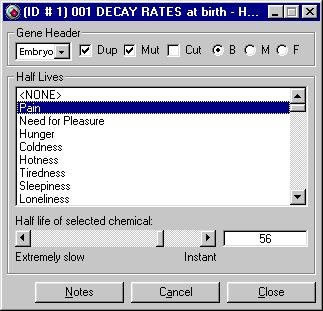
\epsfig {file=img/chemical_halflife.png,width=5.20cm}} % 11.40cm
% 	\caption{Interface for Chemical Half Lives Design}
% 	\label{fig:chemical_halflife}
% \end{figure}
% \end{minipage}
% \subsection{Breakdown}
% \textbf{\textit{Gene Header}} : \emph{The gene header is the same for all genes.}~\\
% \textbf{\textit{Half Lives}}~\\
% \begin{itemize}
% \item[] \textit{Chemical}~\\
%	 Within this listbox you can select any of the 255 different chemicals that may exist within the Norn. The selected chemical will be the one that the rate of decay can be defined for in the controls below this listbox.
% \item[] \textit{Half Life}~\\
%	 This defines the rate at which the selected chemical will decay. It is a number ranging from 0 through to 255. The higher the number the longer it takes for the chemical to drop down to zero. The Genetics Kit only allows certain numbers to be selected and for these numbers it displays an approximate time in seconds.~\\
% This is the time it will take for the chemical to drop from it's value down to zero. The following table shows the number and approximate rate as listed by the genetics kit:
% \end{itemize}
%\begin{longtable}{|p{0.075\textwidth}|p{0.20\textwidth}|p{0.001\textwidth}|p{0.075\textwidth}|p{0.20\textwidth}|}
%	\hline \rowcolor[gray]{0.50} \multicolumn{5}{|c|}{Half lives of chemicals} \\
%	\hline \rowcolor[gray]{0.75} \textbf{Half Life} & \textbf{Approximate Time} & & \textbf{Half Life} & \textbf{Approximate Time} \\ \hline
%	\endfirsthead
%	\hline \rowcolor[gray]{0.50} \multicolumn{5}{|c|}{Half lives of chemicals} \\
%	\hline \rowcolor[gray]{0.75} \textbf{Half Life} & \textbf{Approximate Time} & & \textbf{Half Life} & \textbf{Approximate Time} \\ \hline
%	\endhead
%	\hline 
%	\endfoot
%
%	0 	&	Instantly	 & &	128 &	5 hours \\ \hline
%	8 	&	0.4 seconds	 & &	136 &	10 hours \\ \hline
%	16 	&	1 second	 & &	144 &	20 hours \\ \hline
%	24 	&	3 seconds	 & &	152 &	3 days \\ \hline
%	32 	&	5 seconds	 & &	160 &	6 days \\ \hline
%	40 	&	10 seconds	 & &	168 &	12 days \\ \hline
%	48 	&	20 seconds	 & &	176 &	24 days \\ \hline
%	56 	&	40 seconds	 & &	184 &	48 days \\ \hline
%	64 	&	80 seconds	 & &	192 &	96 days \\ \hline
%	72 	&	2.5 minutes	 & &	200 &	112 days \\ \hline
%	80 	&	5 minutes	 & &	208 &	224 days \\ \hline
%	88 	&	10 minutes	 & &	216 &	448 days \\ \hline
%	96 	&	20 minutes	 & &	224 &	896 days \\ \hline
%	104 &	40 minutes	 & &	232 &	13 years \\ \hline
%	112 &	80 minutes	 & &	240 &	26 years \\ \hline
%	120 &	2.5 hours	 & &	248 &	52 years \\ \hline
%	
%		\hline
%	\caption{Half lives of chemicals}
%	\label{tab:Half_lives_chemicals}\\
%\end{longtable}~\\

%\subsection{Notes}
%I'm assuming by the name of the gene that the rate represents a half-life. So it defines the time it takes for the chemical to drop to half of its current value. It seems to work in this manner anyway.~\\
%\rule{10cm}{0.5mm}~\\

% \clearpage

\section{Initial Concentrations} % CDR -- 
\begin{minipage}{0.5\linewidth}
\subsection{Overview}
This gene controls the amount of chemical that will exist within the norn when it is born (or when the gene is activated?). One gene of this kind exists for each chemical within the norn that requires an initial starting value. I don't know the effects of changing the 'switch on' age. If the age is set to something other than embryo does this mean that an amount of chemical will be injected when the creature reaches that age?~\\
\end{minipage}
\begin{minipage}{0.1\linewidth}\end{minipage}
\begin{minipage}{0.4\linewidth}
\subsection{Dialog Box}
\begin{figure}[H]
	\centerline {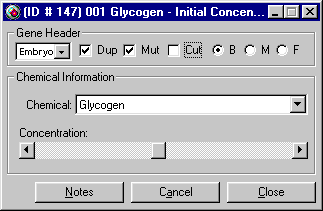
\epsfig {file=img/chemical_initial.png,width=5.20cm}} % 11.40cm
	\caption{Interface for Initial Concentration Design}
	\label{fig:chemical_initial}
\end{figure}
\end{minipage}

\subsection{Breakdown}

\textbf{\textit{Gene Header}} : \emph{The gene header is the same for all genes.}~\\

\textbf{\textit{Chemical Information}}
\begin{itemize}
	\item[] \emph{Chemical} : This will be the chemical that will have the initial concentration defined for this gene.
	\item[] \emph{Concentration} : The amount of chemical to be initially injected into the norn. It is a value from 0 through to 255.
\end{itemize}

\rule{10cm}{0.5mm}~\\

\section{Creature Instinct} % CDR -- 

\subsection{Overview}

An instinct gene provides a way of training the neural net of the norn brain so it will react in certain ways in certain situations. Instinct genes are often used to provide default behavior for things that are very important to the norn. Examples are responding to the verbs typed by the user. These genes do not provide behavior that will always occur. The experiences of the norn during its lifetime can override behavior defined by instincts.~\\

Instincts are processed while a norn is being hatched and while a norn sleeps. It is very important for a norn to get regular sleep so the instincts are constantly reinforced. During this instinct processing time the lobes and neurones define in the gene are set inside the norn brain and the chemical (usually punishment or reward) is processed as if the norn had performed this action.~\\

For example the instinct gene responding to the verb 'come' has the same effect when processed as if the norn had chosen the decision to 'come' when the user typed 'come' and then got a pat from the hand to reward it. This would encourage the norn to do this when awake.

\clearpage

\subsection{Dialog Box}

\begin{figure}[H]
	\centerline {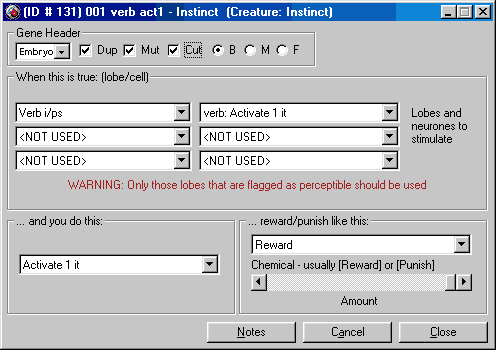
\epsfig {file=img/genes_instinct.png,width=8.75cm}} % 17.498cm
	\caption{Interface for Intincts Design}
	\label{fig:genes_instinct}
\end{figure}

\subsection{Breakdown}

\textbf{\textit{Gene Header}} : \emph{The gene header is the same for all genes.}~\\

\textbf{\textit{When this is true: (lobe/cell)}}~\\

Allows selection of the lobes and cells that will be fired within those lobes. This indicates what the norn will need to perceive before it will decide to take the action defined in the 'and you do this' area. A combination of up to three different lobe/cells may be selected. The Genetics Kit gives a warning that only those lobes marked as perceptible should be used. This makes sense as only the perceptible lobes contribute to forming concepts. Any other lobe will cause this instinct to have no real effect.~\\

The lobes and their perceptible settings are:
\begin{longtable}{|p{0.30\textwidth}|p{0.50\textwidth}|}
	\hline \rowcolor[gray]{0.50} \multicolumn{2}{|c|}{Lobes and perceptible settings} \\
	\hline \rowcolor[gray]{0.75} \textbf{Lobe} & \textbf{Perceptible setting} \\ \hline
	\endfirsthead
	\hline \rowcolor[gray]{0.50} \multicolumn{2}{|c|}{Lobes and perceptible settings} \\
	\hline \rowcolor[gray]{0.75} \textbf{Lobe} & \textbf{Perceptible setting} \\ \hline
	\endhead
	\hline 
	\endfoot

		Drive i/ps 		&	Mutually exclusive \\ \hline
		Stim source i/ps 	&	No \\ \hline
		Verb i/ps 		&	Mutually exclusive \\ \hline
		Noun i/ps 		&	No \\ \hline
		Gen/sense i/ps 		&	Yes \\ \hline
		Decision 		&	No \\ \hline
		Attention 		&	Yes \\ \hline

	\hline
	\caption{Lobes and perceptible settings}
	\label{tab:Lobes_and_perceptible_settings}\\
\end{longtable}~\\~\\

All lobes with a perceptible setting of 'Yes' or 'Mutually Exclusive' qualify as perceptible lobes so they should be able to be used in instincts.~\\

\textbf{\textit{and you do this...}}~\\
This is the decision that the instinct will reinforce when the above lobe/cell combinations are active. Think of it as 'if the above lobe combinations occur then the norn will be more or less likely to make this decision depending on the reward/punish settings defined below. \emph{Valid settings are any of the 16 possible decisions or verbs that the norn can perform: }
	\begin{center} \begin{scriptsize}
		\begin{tabular}{|p{0.5\textwidth}|p{0.5\textwidth}|}
			\hline
			\begin{enumerate}
				\item[0.] Default (\textbf{Stay})
				\item[1.] Activate 1 it (\textbf{Push})
				\item[2.] Activate 2 it (\textbf{Pull})
				\item[3.] Deactivate it (\textbf{Stop})
				\item[4.] Approach it (\textbf{Come})
				\item[5.] Retreat from it (\textbf{Run})
				\item[6.] Get it (\textbf{Get})
				\item[7.] Drop all (\textbf{Drop})
			\end{enumerate}
			&
			\begin{enumerate}
				\item[8.] Say what you need (\textbf{Think})
				\item[9.] Rest (\textbf{Sleep})
				\item[10.] Travel west (\textbf{Left})
				\item[11.] Travel east (\textbf{Right})
				\item[12.] Decision12
				\item[13.] Decision13
				\item[14.] Decision14
				\item[15.] Decision15
			\end{enumerate} \\ \hline
		\end{tabular}
	\end{scriptsize} \end{center}~\\

\textbf{\textit{reward/punish like this}}~\\
This is where you select the chemical and amount of that chemical that will be injected into the norn when the above settings are made and the instinct processed. Although any of the 256 chemicals can be selected the only two that really make sense are 'Reward' or 'Punish'.~\\

If 'Reward' is selected then the norn will be rewarded and encouraged to perform the action. If 'Punish' is selected then the norn will be discouraged and be less likely to perform the action defined.

\subsection{Notes}

Remember that instincts are only processed when a norn is born and while it sleeps. Too many instinct genes could cause a lot more sleep or longer sleep to be required for all the instincts to be processed. It may pay to have the more important instincts to be the lower numbered genes (as it appears to cycle through in gene number order).~\\

Some instinct genes appear to use the Stim source lobe as an input even though it is not a perceptible lobe. I'm in the process of testing whether these instincts actually work as I suspect they may not. It depends whether the instinct processing mechanism still considers it as perceptible as the Stim source lobe feeds into the Attention lobe which is perceptible. Some research is needed here.~\\

Although only 'Reward' and 'Punish' currently make sense for chemicals, others could be useful in genetically modified norns with different brain/chemical structures. There is scope for some interesting experimentation there. Only three lobe/cell combinations can be defined. This appears to match the number of dendrite links between the perception lobe and the concept lobe in a standard hatchery norn. These norns allow up to three perceptions to form a concept.~\\

% If you can provide any additional information to help document this gene please let me know (chris@double.co.nz).~\\

% \rule{10cm}{0.5mm}~\\

\section{Creature Stimulus} % CDR -- 
\begin{minipage}{0.5\linewidth}
\subsection{Overview}
A stimulus is an event that happens to the norn that it can react to in some manner. The stimulus gene allows the reaction to these stimuli to be defined. This can range from chemicals being injected to cell values in brain lobes being adjusted. There are a number of stimulus responses that are hard coded within the Creatures program. The stimulus genes that are created override these hard coded responses giving a lot of flexibility in determining how the creature will react to the world.~\\
\end{minipage}
\begin{minipage}{0.1\linewidth}\end{minipage}
\begin{minipage}{0.4\linewidth}
\subsection{Dialog Box}
\begin{figure}[H]
	\centerline {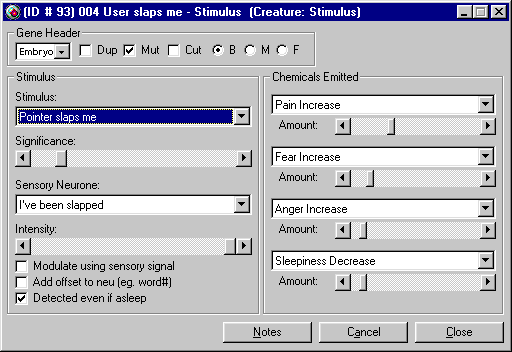
\epsfig {file=img/gene_stimulus.png,width=5cm}} % 18.00cm
	\caption{Interface for Stimulus Design}
	\label{fig:genes_stimulus}
\end{figure}
\end{minipage}~\\

\clearpage

\subsection{Breakdown}

\textbf{\textit{Gene Header}} : \emph{The gene header is the same for all genes.}~\\

\textbf{\textit{Stimulus}}
\begin{itemize}
\item[] \emph{Stimulus} : The stimulus that this gene is attached to. When this stimulus occurs then the effects defined by this gene will be applied. The following stimuli are available:
	\begin{center} \begin{scriptsize}
		\begin{tabular}{|p{0.30\textwidth}|p{0.30\textwidth}|p{0.30\textwidth}|}
			\hline
			\begin{itemize}
				\item Disappointment
				\item Pointer pats me
				\item Creature pats me
				\item Pointer slaps me
				\item Creature slaps me
				\item It is approaching
				\item It is retreating
				\item I bump into wall
				\item Object comes into view
			\end{itemize}
			&
			\begin{itemize}
				\item Unrecognised word
				\item Heard user speak
				\item Heard creature speak
				\item I am quiescent (periodic)
				\item I've activated1
				\item I've activated2
				\item I've deactivated
				\item I am approaching (periodic)
				\item I have retreated
			\end{itemize}
			&
			\begin{itemize}
				\item I have got
				\item I have dropped
				\item I've stated need
				\item I am resting (periodic)
				\item I am sleeping (periodic)
				\item I am traveling (periodic)
				\item spare action 1-4
				\item Involuntary action 0-7
			\end{itemize} \\ \hline
		\end{tabular}
	\end{scriptsize} \end{center}~\\
 
\item[] \emph{Significance} : The amount will be increased the neuron relating to the object that caused the stimulus in the Stimulus/Source lobe. This has the effect of making the object appear more interesting and so it is more likely to be looked at. The neuron that gets nudged by this amount appears to differ for each Stimuli (a neuron for each object type in view). 
\item[] \emph{Sensory Neurone} : Identifies a cell in the General Sense lobe which will get adjusted by the value given in the 'Intensity' field described below. This allows setting up what the norn can actually sense from the stimuli going on around it. The following cells are available and map directly to cells in the general sense lobe:
	\begin{center} \begin{scriptsize}
\begin{tabular}{|p{0.30\textwidth}|p{0.30\textwidth}|p{0.30\textwidth}|}
		\hline
			\begin{itemize}
				\item $<$none$>$
				\item I've been patted
				\item I've been slapped
				\item I've bumped a wall
				\item I am near a wall
				\item I am in a vehicle
				\item User has spoken
				\item Creature has spoken
			\end{itemize}
			&
			\begin{itemize}
				\item Own kind has spoken
				\item Audible event
				\item Visible event
				\item It is approaching
				\item It is retreating
				\item It is near to me
				\item It is active
			\end{itemize}
			&
			\begin{itemize}
				\item It is an object
				\item It is a creature
				\item It is my sibling
				\item It is my parent
				\item It is my child
				\item It is opposite sex
				\item spare 2-13
			\end{itemize} \\
		\hline
		\end{tabular}
	\end{scriptsize} \end{center}~\\
 
\item[] \emph{Intensity} : This is the amount by which the particular sensory neurone will be increased by. So if the value here is '50' and the current value of the particular neurone is '25' then when this stimuli occurs the sensory neurone will fire at a value of about '75'.
\item[] \emph{Modulate using sensory signal} : From what I can gather this means that the 'significance' value applied to the stimulus source lobe is first modulated by the value of the neuron associated with the stimulus. I'm not exactly sure what particular value it is modulated by and perhaps it is best explained by describing some of the results I've gotten through experimentation. See the notes section for details. If anyone can provide a clearer explanation I'd appreciate an email.
% \item[] \emph{Add offset to neu (eg. word\#)} : 
\item[] \emph{Detected even if asleep} : If the norn is asleep and this option is unchecked then the stimulus will be ignored and none of the effects will be applied. If it is checked then the gene will be processed even if the norn is sleeping.
\end{itemize}~\\

\textbf{\textit{Chemicals Emitted}}~\\
Up to four chemicals can be selected along with a particular amount of that chemical to be injected. When the stimulus occurs the defined amount of these chemicals will be injected into the norn.

\clearpage

%%%%% \section{CDR -- State Variable Rules (SVR)}

\section{Brain Lobes -- \textit{Creatures 1}} % CDR -- 

% $<$\textit{http://www.double.co.nz/creatures/brainlobes/lobes.htm}$>$

\subsection{Overview}

The norn brain is divided into a number of lobes. In the standard Creatures 1 genome there are nine and in the Creatures 2 genome there are ten.~\\

The brain lobes numbered from 0 through to 8 are hard coded by the Creatures executable to perform a particular function. For example, firing a cell in lobe 6 (decision) causes the creature to perform a particular action. The genetic definition of that lobe then defines what happens as a result of this firing. In the case of the decision lobe it is to manage the learning of whether the decision was a good one or a bad one.~\\

The higher numbered brain lobes are not controlled by the Creatures executable at all. They are controlled completely through genetics. So for these lobes to do anything a system of receptors, emitters and dendrites must be set up to fire cells or act upon cells firing.~\\

The purpose and function of each lobe is outlined below with descriptions.
\begin{itemize}
\item[\textbf{Lobe 0 -- Perception}]
	Copies data from other lobes to form a composite lobe containing all cells that can be used to form concepts.
\item[\textbf{Lobe 1 -- Drive}]
	Holds the current values of the creatures drives.
\item[\textbf{Lobe 2 -- Stimulus source}]
	Stimulating objects near to the creature cause cells in this lobe to fire so the creature can react to them.
\item[\textbf{Lobe 3 -- Verb}]
	Cells in this lobe fire when the user types a verb in the speech box.
\item[\textbf{Lobe 4 -- Noun}]
	Cells in this lobe fire when the user types a noun in the speech box or types 'look' with the hand hovering over an object.
\item[\textbf{Lobe 5 -- General Sensory}]
	Indicates events that the norn can sense. Usually caused by the effects of processing stimulus genes.
\item[\textbf{Lobe 6 -- Decision}]
	An output lobe. By firing a cell in this lobe you cause the creature to perform a particular action.
\item[\textbf{Lobe 7 -- Attention}]
	An output lobe. By firing a cell in this lobe you cause the creature to look at a particular object.
\item[\textbf{Lobe 8 -- Concept}]
	A storehouse of memories and concepts.
\item[\textbf{Lobe 9 -- Regulator}]
	This lobe provides feedback loops for biochemical regulations. % This lobe is not really part of the norn brain/decision mechanism as such. It provides functionality similar to the hunger/glycogen floating receptor emitters used by the norns in the Creatures 1 life kit. Special thanks to Lis Morris for the description of this lobe.
\end{itemize}~\\

While the lobes have individual functionality it is how they work together that results in the norn brain working. There lobes combine to form a couple of main learning systems that are described briefly in the individual lobe descriptions but will be covered in more detail in future updates:
\begin{itemize}
	\item Attention seeking system
	\item Concept learning system
	\item Decision learning system
\end{itemize}~\\

%% \begin{minipage}[ht]{0.45\textwidth}
	%% \def\captionof#1#2{{\def\@captype{#1}#2}}
	%% attention aux flottants dans les flottants !!
	\begin{table}[ht]
		\begin{center} \begin{scriptsize}
		\begin{tabular}{|c|c|c|c|c|c|c|}
			\hline
		\rowcolor[gray]{0.75} 
		Number	&	Name	&	X	&	Y	&	Width	&	Height	&	Neurones \\ \hline
		0	&	Perception	&	4	&	13	&	7		&	16		&	112 \\ \hline
		1	&	Drive		&	34	&	30	&	8		&	2		&	16 \\ \hline
		2	&	Source		&	15	&	24	&	8		&	5		&	40 \\ \hline
		3	&	Verb		&	37	&	24	&	8		&	2		&	16 \\ \hline
		4	&	Noun		&	21	&	3	&	20		&	2		&	40 \\ \hline
		5	&	Gen. Sense	&	32	&	34	&	8		&	4		&	32 \\ \hline
		6	&	Decision	&	53	&	15	&	1		&	16		&	16 \\ \hline
		7	&	Attention	&	44	&	30	&	5		&	8		&	40 \\ \hline
		8	&	Concept		&	12	&	6	&	40		&	16		&	640 \\ \hline
		\end{tabular}
		\caption[Norn Lobes for \emph{Creatures 1}]{Norn Lobes for \emph{Creatures 1} \\ \emph{Description of lobes positions and size,  brain is $64*48$. The Regulator lobe, \textnormal{SandraBellum}, is not present. } } % ~\cite{genornics}. } }
		\end{scriptsize} \end{center}
		\label{tab:nornsLobesPositionsCreatures1}
	\end{table}
%% \end{minipage} \hfill \begin{minipage}[ht]{0.45\textwidth}
	\begin{table}[ht]
		\begin{center} \begin{scriptsize}
		\begin{tabular}{|c|c|c|c|c|c|c|}
			\hline
		\rowcolor[gray]{0.75} 
		Number	&	Name	&	X	&	Y	&	Width	&	Height	&	Neurones \\ \hline
		0	&	Perception	&	1	&	13	&	7		&	16		&	112 \\ \hline
		1	&	Drive		&	34	&	36	&	6		&	3		&	18 \\ \hline
		2	&	Source		&	15	&	32	&	8		&	5		&	40 \\ \hline
		3	&	Verb		&	37	&	32	&	8		&	2		&	16 \\ \hline
		4	&	Noun		&	21	&	1	&	20		&	2		&	40 \\ \hline
		5	&	Gen. Sense	&	32	&	40	&	8		&	4		&	32 \\ \hline
		6	&	Decision	&	62	&	15	&	1		&	16		&	16 \\ \hline
		7	&	Attention	&	44	&	36	&	5		&	8		&	40 \\ \hline
		8	&	Concept		&	11	&	5	&	40		&	16		&	640 \\ \hline
		9	&	Regulator	&	4	&	40	&	16		&	1		&	16 \\ \hline
		\end{tabular}
		\end{scriptsize} \end{center}
		\caption[Norn Lobes for \emph{Creatures 2}]{Norn Lobes for \emph{Creatures 2} \\ \emph{Description of lobes positions and size,  brain is $64*48$. } } % ~\cite{genornics}. } }
		\label{tab:nornsLobesPositionsCreatures2}
	\end{table}
%% \end{minipage} ~\\

\begin{minipage}{0.5\textwidth}
\begin{figure}[H]
	\centerline {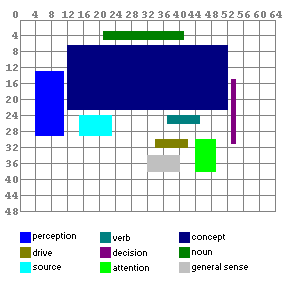
\epsfig {file=img/brainmapCreatures1.png,width=7cm}}
	\caption{Creatures 1 Brain Map. } % ~\cite{genornics}}
	\label{fig:Creatures1BrainMap}
\end{figure}
\end{minipage}
\begin{minipage}{0.1\textwidth}\end{minipage}
\begin{minipage}{0.5\textwidth}
\begin{figure}[H]
	\centerline {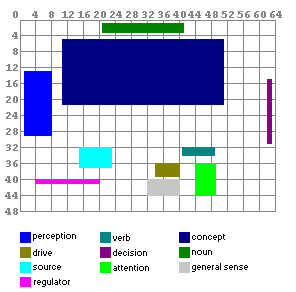
\epsfig {file=img/brainmapCreatures2.png,width=7cm}}
	\caption{Creatures 2 Brain Map. } % ~\cite{genornics}}
	\label{fig:Creatures2BrainMap}
\end{figure}
\end{minipage}

% \clearpage

\subsection{Lobe 0 -- Perception Lobe}

% \emph{To be completed. \underline{see special section} }

The purpose of the perception lobe appears to be to summarise everything that a norn can 'perceive' into one brain lobe so the norn can eventually store concepts and memories based upon these perceptions (done in the concept lobe). This tutorial attempts to answer the questions about how the perceptible lobes are summarised into the perception lobe and how to work out what each cell of the perception lobe means.~\\

The usual method of passing cell information from one lobe to another is through wiring up dendrites. Using dendrites can only summarise information from two other brain lobes (the D0 and D1 dendrite connections). With the perception lobe there is more than two lobes that need to be summarised so it appears a mechanism specifically for dealing with the perception lobe was built.~\\

Brain lobes are marked as 'Yes', 'No' or 'Mutually Exclusive' to be copied in the Perception lobe. The brain lobes that are marked as 'Yes' or 'Mutually exclusive' in an original norn are:
\begin{longtable}{|p{0.25\textwidth}|p{0.15\textwidth}|p{0.65\textwidth}|}
	\hline \rowcolor[gray]{0.50} \multicolumn{3}{|c|}{Copied Lobes in Perception} \\
	\hline \rowcolor[gray]{0.75} \textbf{Lobe} & \textbf{Size} & \textbf{Data copied to perception lobe?} \\ \hline
	\endfirsthead
	\hline \rowcolor[gray]{0.50} \multicolumn{3}{|c|}{Copied Lobes in Perception} \\
	\hline \rowcolor[gray]{0.75} \textbf{Lobe} & \textbf{Size} & \textbf{Data copied to perception lobe?} \\ \hline
	\endhead
	\hline 
	\endfoot
	Drive lobe		&	16 &	Mutually exclusive \\ \hline
	Verb lobe		&	16 &	Mutually exclusive \\ \hline
	General sense lobe	&	32 &	Yes \\ \hline
	Attention lobe 		&	40 &	Yes \\ \hline
	\caption{Copied Lobes in Perception}
	\label{tab:Copied_Lobes_in_Perception}\\
\end{longtable}

\clearpage

The perception lobe must have a number of cells equal to or greater than the total number of cells in all lobes marked as 'Yes' or 'Mutually exclusive'. The total number of cells in the above lobes equals 104. The size of the perception lobe is 112 so there is a little room to spare there.

\subsection{Lobe 1 -- Drive Lobe}

This lobe holds the current state of the creatures drives (such as hunger, pain, etc). It directly maps to the particular drive chemicals that can be viewed using the science kit. Changing the values of the cells directly in this lobe using CAOS is unlikely to have much of an effect on the norn as the cells are directly set by receptors in the genome. This means that whatever values you manipulate with CAOS commands will be immediately overwritten with the current value of the drive chemical. To change drive values it would seem to be best to change the values of the chemicals either directly or through the drive increaser/reducer chemicals. \emph{The size of the lobe was increased in Creatures 2 to cater for the addition of more drives. The cell values are outlined in the following table:}
\begin{longtable}{|p{0.15\textwidth}|p{0.40\textwidth}|p{0.40\textwidth}|}
	\hline \rowcolor[gray]{0.50} \multicolumn{3}{|c|}{Drive Lobe Data Entries \textit{Drives} } \\
	\hline \rowcolor[gray]{0.75} \textbf{Cell} & \textbf{Creatures 1} & \textbf{Creatures 2} \\ \hline
	\endfirsthead
	\hline \rowcolor[gray]{0.50} \multicolumn{3}{|c|}{Drive Lobe Data Entries \textit{Drives} } \\
	\hline \rowcolor[gray]{0.75} \textbf{Cell} & \textbf{Creatures 1} & \textbf{Creatures 2} \\ \hline
	\endhead
	\hline 
	\endfoot

0	&	Pain			&	Pain			 \\ \hline
1	&	Need for Pleasure	&	Need for Pleasure	 \\ \hline
2	&	Hunger			&	Hunger			 \\ \hline
3	&	Coldness		&	Coldness		 \\ \hline
4	&	Hotness			&	Hotness			 \\ \hline
5	&	Tiredness		&	Tiredness		 \\ \hline
6	&	Sleepiness		&	Sleepiness		 \\ \hline
7	&	Loneliness		&	Loneliness		 \\ \hline
8	&	Overcrowdedness		&	Overcrowdedness		 \\ \hline
9	&	Fear			&	Fear			 \\ \hline
10	&	Boredom			&	Boredom	 		 \\ \hline
11	&	Anger			&	Anger	 		 \\ \hline
12	&	Sexdrive		&	Sexdrive		 \\ \hline
13	&	\emph{Not Allocated}	&	Injury	 		 \\ \hline
14	&	\emph{Not Allocated}	&	Suffocation		 \\ \hline
15	&	\emph{Not Allocated}	&	Thirst			 \\ \hline
16	&	\emph{No such cell}	&	Stress			 \\ \hline
17	&	\emph{No such cell}	&	\emph{Not Allocated}	 \\ \hline
	\caption{Drive Lobe Data Entries \textit{Drives} }
	\label{tab:Drive_Lobe_Data_Entries}\\
\end{longtable}

The drive lobe feeds into the Perception lobe and is marked as mutally exclusive. This means that, at most, one cell from the drive lobe will exist in any given concept that the creature forms. So the creature cannot form the concept of 'hot and hungry'. Only 'hot' or 'hungry' or a combination of these drives with some other perception lobe cell. 

\subsection{Lobe 2 -- Stimulus Source Lobe}

Cells in this lobe are activated directly by the Creatures executable. The lobe has 40 cells - one for each object classification in Creatures. -- Each cell relates to a particular object classification. The cell fires for a given object if that object is within the creatures line of sight and is stimulating in some manner. Stimulus genes can be used to modify this lobe indirectly to indicate whether the object is more or less stimulating. The higher the cell value in a particular cell, the more stimulating that object currently is.~\\

It is a 'winner takes all' lobe, meaning that the highest firing cell will be the only firing cell. This means that the most stimulating object in the area of the norn will be the only object that will appear to be stimulating to the norn. The State value for all the cells is calculated and the cell with the highest state will be the only one with an output value - indicating that it is firing.~\\

% In Creatures 1 this lobe has no state variable rule indicating that the state values are directly set by the executable or some other means (like cobs or genetics).~\\

% In Creatures 2 there is a state variable rule set to '$random:0:chem 5:PLUS:state:end$'. This means that the state is calculated by getting the previous state value and adding a random number (ranging from 0 through to the value of chemical 5) to it. Brain chemical 5 is set via a receptor gene that reacts to the chemical Triptophan (169). This receptor injects brain chemical 5 at the same level as the Triptophan chemical exists in the norn. Triptophan is described in the strategy guide as causing creatures to see objects that are not really there - a hallucinogenic. This state rule is how it works. If an amount of 100 units of Triptophan exists in the norn then 100 units of brain chemical 5 will exist. This will cause all cells in the stimulus source lobe to have their state calculated as the previous state plus a random number from 0 to 100. So the creature can end up thinking things are there when they are really not.~\\

% \rule{10cm}{0.5mm}~\\~\\

The following table outlines the cell values for this lobe:
\begin{longtable}{|p{0.15\textwidth}|p{0.40\textwidth}|p{0.40\textwidth}|}
	\hline \rowcolor[gray]{0.50} \multicolumn{3}{|c|}{Source Lobe Data Entries} \\
	\hline \rowcolor[gray]{0.75} \textbf{Cell} & \textbf{Creatures 1} & \textbf{Creatures 2} \\ \hline
	\endfirsthead
	\hline \rowcolor[gray]{0.50} \multicolumn{3}{|c|}{Source Lobe Data Entries} \\
	\hline \rowcolor[gray]{0.75} \textbf{Cell} & \textbf{Creatures 1} & \textbf{Creatures 2} \\ \hline
	\endhead
	\hline 
	\endfoot
	
0	&	Current norn		&	Current norn	 \\ \hline
1	&	Hand			&	Hand		 \\ \hline
2	&	Call button		&	Call Button	 \\ \hline
3	&	Water			&	Nature	 	 \\ \hline
4	&	Plant			&	Plant		 \\ \hline
5	&	Egg			&	Egg		 \\ \hline
6	&	Food			&	Food		 \\ \hline
7	&	Drink			&	Drink		 \\ \hline
8	&	Vendor			&	Dispenser	 \\ \hline
9	&	Music			&	Implement	 \\ \hline
10	&	Animal			&	Cliff Edge	 \\ \hline
11	&	Fire			&	Detritus	 \\ \hline
12	&	Shower			&	Medicine	 \\ \hline
13	&	Toy			&	Toy	 	 \\ \hline
14	&	Bigtoy			&	Weather	 	 \\ \hline
15	&	Weed			&	Badplant	 \\ \hline
16	&	Incubator		&	Nest		 \\ \hline
17	&	Blackboard word 33	&	Badbug		 \\ \hline
18	&	Blackboard word 34	&	Bug		 \\ \hline
19	&	Blackboard word 35	&	Badcritter	 \\ \hline
20	&	Blackboard word 36	&	Critter		 \\ \hline
21	&	Blackboard word 37	&	Seed		 \\ \hline
22	&	Blackboard word 38	&	Leaf		 \\ \hline
23	&	Blackboard word 39	&	Root		 \\ \hline
24	&	Blackboard word 40	&	Flower		 \\ \hline
25	&	Blackboard word 41	&	Fruit		 \\ \hline
26	&	Mover			&	Mover		 \\ \hline
27	&	Lift			&	Lift		 \\ \hline
28	&	Computer		&	Computer	 \\ \hline
29	&	Fun			&	Mediabox	 \\ \hline
30	&	Bang			&	Message		 \\ \hline
31	&	Blackboard word 47	&	Leftright	 \\ \hline
32	&	Blackboard word 48	&	Incubator	 \\ \hline
33	&	Blackboard word 49	&	Teleporter	 \\ \hline
34	&	Blackboard word 50	&	Blackboard word 50	 \\ \hline
35	&	Blackboard word 51	&	Machine		 \\ \hline
36	&	Norn			&	Norn		 \\ \hline
37	&	Grendel			&	Grendel		 \\ \hline
38	&	Ettin			&	Ettin		 \\ \hline
39	&	Shee			&	Shee		 \\ \hline

		\hline
	\caption{Source Lobe Data Entries }
	\label{tab:Source_Lobe_Data_Entries}\\
\end{longtable}

The cell numbers appear to relate to the genus numbers for Objects (COB). So an Object with a genus value of 21 sitting near a norn in Creatures 2 will stimulate cell 21 in the norn, making it think a Seed is nearby. 

\clearpage

\subsection{Lobe 3 -- Verb Lobe}

The Verb lobe is another lobe that is controlled directly by the Creatures executable. Whenever a verb is entered by the user in the speech box of Creatures then the cell associated with this verb will be fired in this lobe. It's also possible that verbs mentioned by other creatures nearby could fire cells in this lobe but I haven't checked into this yet. -- The following table outlines the cell values for this lobe:
\begin{longtable}{|p{0.15\textwidth}|p{0.40\textwidth}|p{0.40\textwidth}|}
	\hline \rowcolor[gray]{0.50} \multicolumn{3}{|c|}{Verb Lobe Data Entries} \\
	\hline \rowcolor[gray]{0.75} \textbf{Cell} & \textbf{Creatures 1} & \textbf{Creatures 2} \\ \hline
	\endfirsthead
	\hline \rowcolor[gray]{0.50} \multicolumn{3}{|c|}{Verb Lobe Data Entries} \\
	\hline \rowcolor[gray]{0.75} \textbf{Cell} & \textbf{Creatures 1} & \textbf{Creatures 2} \\ \hline
	\endhead
	\hline 
	\endfoot
0	&	Quiescent	&	Quiescent	 \\ \hline
1	&	Push		&	Push	 	 \\ \hline
2	&	Pull		&	Pull		 \\ \hline
3	&	Stop		&	Stop		 \\ \hline
4	&	Come		&	Come		 \\ \hline
5	&	Run		&	Run		 \\ \hline
6	&	Get		&	Get		 \\ \hline
7	&	Drop		&	Drop		 \\ \hline
8	&	Think		&	What		 \\ \hline
9	&	Sleep		&	Sleep		 \\ \hline
10	&	Left		&	Left		 \\ \hline
11	&	Right		&	Right		 \\ \hline
12	&	\emph{Not Allocated}	&	Eat	 \\ \hline
13	&	\emph{Not Allocated}	&	Hit	 \\ \hline
14	&	\emph{Not Allocated}	&	\emph{Not Allocated}	 \\ \hline
15	&	\emph{Not Allocated}	&	\emph{Not Allocated}	 \\ \hline
	\caption{Verb Lobe Data Entries }
	\label{tab:Verb_Lobe_Data_Entries}
\end{longtable}

The word that was learnt for the particular verb slot is what must be typed in for that cell in this lobe to fire. So if the Norn knows 'Push' as 'foo' then typing 'foo' will fire the particular cell. If a complete command is entered like 'alice eat food' then cell 12 in this lobe (for eat) will fire along with the 'food' cell in the noun lobe.

\subsection{Lobe 4 -- Noun Lobe}

Cells in the noun lobe are fired when a noun is entered by the user using the speech box of the Creatures executable. It works the same as the verb lobe described above but it is for the objects rather than the action to be performed on the object. It is another lobe controlled directly by the Creatures executable.~\\

The noun lobe will also fire if the user moves the hand over an object and types the command 'look'. This causes the cell for that particular object to fire in the noun lobe. The result of this is the norn usually ends up looking at the requested object. See the description of the Attention lobe for details on how this works.

\subsection{Lobe 5 -- General Sensory Lobe}

The cells in this lobe define what the norn can currently sense in the environment. Where the stimulus source lobe is the objects within the environment this lobe is various environmental factors relating to those objects. For example, cells for detecting that the creatures has just been patted, slapped, fallen, whether nearby creatures are the same sex, same species, the parents of the current creature, etc.~\\

The cells in this lobe can be manipulated using the stimulus genes. When a particular stimulus occurs (either by the Creatures executable or using CAOS in a COB) the stimulus gene is activated. That gene can then cause a general sensory lobe cell to fire at a particular intensity so the norn can react or learn from that stimulus.~\\

% The lobe has a state variable rule of 'state:end' which means that the state is calculated as being the previous state value the leakage rate applied to it. This type of state rule usually indicates that the brain lobe is only modified via genetics rather than the Creatures executable itself.~\\

The lobe is copied to the Perception lobe allowing the cells to be used for forming concepts. This means that a norn can learn whether 'approaching an edge' is good or bad for example.~\\

The following table outlines the cell values for the General Sensory Lobe :
\begin{longtable}{|p{0.15\textwidth}|p{0.40\textwidth}|p{0.40\textwidth}|}
	\hline \rowcolor[gray]{0.50} \multicolumn{3}{|c|}{General Senses Lobe Data Entries} \\
	\hline \rowcolor[gray]{0.75} \textbf{Cell} & \textbf{Creatures 1} & \textbf{Creatures 2} \\ \hline
	\endfirsthead
	\hline \rowcolor[gray]{0.50} \multicolumn{3}{|c|}{General Senses Lobe Data Entries} \\
	\hline \rowcolor[gray]{0.75} \textbf{Cell} & \textbf{Creatures 1} & \textbf{Creatures 2} \\ \hline
	\endhead
	\hline 
	\endfoot
0	&	I've been patted	&	I've been patted	 \\ \hline
1	&	I've been slapped	&	I've been slapped	 \\ \hline
2	&	I've bumped into a wall	&	I've bumped into a wall	 \\ \hline
3	&	I am near a wall	&	I am near a wall	 \\ \hline
4	&	I am in a vehicle	&	I am in a vehicle	 \\ \hline
5	&	User has spoken		&	User has spoken		 \\ \hline
6	&	Creature has spoken	&	Creature has spoken	 \\ \hline
7	&	Own kind has spoken	&	Own kind has spoken	 \\ \hline
8	&	Audible event		&	Audible event		 \\ \hline
9	&	Visible event		&	Visible event		 \\ \hline
10	&	It is approaching	&	It is approaching	 \\ \hline
11	&	It is retreating	&	It is retreating	 \\ \hline
12	&	It is near me		&	It is near me		 \\ \hline
13	&	It is active		&	It is active		 \\ \hline
14	&	It is an object		&	It is an object		 \\ \hline
15	&	It is a creature	&	It is a creature	 \\ \hline
16	&	It is my sibling	&	It is my sibling	 \\ \hline
17	&	It is my parent		&	It is my parent		 \\ \hline
18	&	It is my child		&	It is my child		 \\ \hline
19	&	It is opposite sex	&	It is opposite sex	 \\ \hline
20	&	\emph{Not Allocated}	&	It has pushed me	 \\ \hline
21	&	\emph{Not Allocated}	&	It has hit me		 \\ \hline
22	&	\emph{Not Allocated}	&	\emph{Not Allocated}	 \\ \hline
23	&	\emph{Not Allocated}	&	\emph{Not Allocated}	 \\ \hline
24	&	\emph{Not Allocated}	&	\emph{Not Allocated}	 \\ \hline
25	&	\emph{Not Allocated}	&	\emph{Not Allocated}	 \\ \hline
26	&	\emph{Not Allocated}	&	\emph{Not Allocated}	 \\ \hline
27	&	\emph{Not Allocated}	&	\emph{Not Allocated}	 \\ \hline
28	&	\emph{Not Allocated}	&	Approaching an edge	 \\ \hline
29	&	\emph{Not Allocated}	&	Retreating from an edge	 \\ \hline
30	&	\emph{Not Allocated}	&	Falling through the air	 \\ \hline
31	&	\emph{Not Allocated}	&	Hitting the ground post fall	 \\ \hline
	\caption{General Senses Lobe Data Entries }
	\label{tab:General_Senses_Lobe_Data_Entries}\\
\end{longtable}

\subsection{Lobe 6 -- Decision Lobe}

Each cell in the decision lobe relates to a particular action that the norn can perform. These actions are the same as the verbs in the verb lobe. See the table in that lobe for descriptions of the individual cells.~\\

The Verb lobe is an input lobe - it receives input typed in from the user. The decision lobe is an output lobe. By firing a cell in the decision lobe the Creatures executable will be directed to make the norn perform the particular decision related to the cell being fired. By manually firing cells in this lobe you can force a norn to perform certain decisions. This is how the 'shove' mode of the hand works. When you have the hand in 'shove' mode, pressing a norn results in either the 'left' (cell 10) or 'right' (cell 11) cell to be activated. This will usually cause the norn to move left or right.~\\

%% \clearpage

% ====>> % The decision lobe has a learning mechanism built into it. It will learn what decisions are the best ones to make when certain concepts are present. I call this the decision learning system and it will be described elsewhere as it is quiet detailed.~\\

The decision lobe is connected to the concept lobe using type 0 and type 1 dendrites. 128 dendrites of each type connect to the concept lobe. Each dendrite link is therefore linked to a particular concept. A concept is a combination of perceptable things (eg. hungry and looking at food, tired, sleepy and just been patted by the hand, etc).~\\

The type 0 dendrites link from decision lobe cells to the 128 concept lobe cells indicate that that particular decision is good if those particular concepts are active. This means that if the concepts become active then the norn will be more likely to choose that decision over other decisions.~\\

The type 1 dendrites link from decision lobe cells to the 128 concept lobe cells indicate that that particular decision is bad if those particular concepts are active. This means that if the concepts become active then the norn will be less likely to choose that decision over other decisions.

% See the upcoming description of the decision learning system for more detail.

\subsection{Lobe 7 -- Attention Lobe}

Each cell in the attention lobe relates to a particular object classification in the same manner as the Stimulus Source lobe and the Noun lobe. See the table in those lobe descriptions for the meanings of the individual cells.~\\

The Simulus Source and Noun lobes are input lobes - they receive input from the environment. The attention lobe is an output lobe. When a cell fires in the attention lobe then the Creatures executable is told to make the norn look at a particular object. If you manually fire a cell in this lobe you will see the 'Creatures View' in the game change to whatever object corresponds to the cell you fired.~\\

Like the stimulus source lobe, it is a 'winner takes all' lobe. This means that only one cell will actually fire - the cell with the highest state value. This makes sense as the norn can only look at one object at a time. The attention lobe copies its information to the perception lobe enabling the current object being looked at to be used in formating concepts. --- A mechanism that I call the attention seeking system exists that makes the norn look at the most stimulating object nearby or an object that the user recently asked the norn to look at (by typing 'look' or entering the name of the object). This system works by using dendrite connections from the attention lobe to the stimulus source and noun lobes.~\\

There is one type 0 dendrite linking each cell in the attention lobe to the equivalent cell in the stimulus source lobe. This means that if a cell fires in the stimulus source lobe the value of the firing can be used in state variable calculations in the attention lobe.~\\

There is one type 1 dendrite linking each cell in the attention lobe to the equivalent cell in the noun lobe. Effectively there is a link passing information from the stimulus source and the noun lobe through to the attention lobe.

% The attention lobe has the following state variable rule: '$state:plus:type0:plus:type1:end$'. This rule is used when calculating the state value of each cell in the attention lobe. So for cell 0 it will take the current state value and add the value of cell 0 from the type 0 dendrites (which will be cell 0 in the stimulus source lobe) and add the value of cell 0 from the type 1 dendrites (cell 0 in the noun lobe). So the calculation is current state plus the sum of whatever stimulation comes from the other two lobes. The cell in the Attention lobe with the highest state then fires at this level (due to it being a winner takes all lobe).~\\

% From this it can be seen that a creature will always look at the most stimulating object, taking into account anything the user has typed as well. It never actually decides what to look at. No learning takes place in the attention seeking system. This is one of the limitations that I see with the current norn brain setup. It can be very hungry but unless it is actually looking at food it will never eat it and it can never decide to look at food - it can only look at it if it happens to be the most stimulating object in the area.~\\

% The original Creatures 1 release in the UK had the following state variable rule in this lobe: '$state:plus:type0:end$'. The noun lobe connection was inadvertantly left out. Usually this would mean the norns would not listen to commands typed by the user. I've heard from sources that the Creatures executable was modified to work around this problem before the game hit the shelves. Newly patched versions of the game don't exhibit this problem.

% The attention lobe copies its information to the perception lobe enabling the current object being looked at to be used in formating concepts.~\\

\subsection{Lobe 8 -- Concept Lobe}

% \emph{To be completed. }~\\

By far the largest region of a norn's brain is used to store memories of the events that occur over its lifetime. This region is called Concept Space, and seems to be involved in the collation and organization of a norn's perceptions and experiences. We know that the neurons in this region are very mobile, and are constantly reconnecting themselves to the main sensory lobe in response to new experiences. Artificial stimulation of these neurons can trigger outward behavior, but it is not certain what the relationship is between a given neuron and the behavior it produces. The Concept lobe is the biggest lobe in a Norn's brain. In Creatures 1 it has a size of 640 neurons.~\\

%% \clearpage

This lobe receives input signals from the different sense lobes (via the perception lobe in C1 and C2). One neuron of this lobe may have between one and three input dendrites. All inputs of a single neuron are calculated together with a logical AND operation. This is why this lobe is also called "Combination lobe" in Creatures 3 -- it simply combines up to three different inputs to one output. Possible meanings may be: "I am hungry AND I see food" or "There is a creature AND it is a Grendel AND it is approaching".~\\

%% \clearpage

The dendrite's strength is increased by the "reward" chemical and decreased by the "punish" chemical. Dendrites with a strength near zero may migrate to connect to different active input signals, making new random connections possible. The output of the neurons in this lobe is passed to the decision lobe. These dendrites may get positive or negative strength values, so they represent what the creature should or should not do in a certain situation.~\\

\subsection{Lobe 9 -- Regulator Lobe}

% Lis Morris, co-creator of the Canny norns, was kind enough to supply the details of the Regulator lobe for me. Thanks Lis!~\\

The regulator lobe (or Sandrabellum named after Sandra Linkletter / slink who created it) is not part of the norn attention, concept, and decision mechanism. It supplies functionality similar to that of the floar receptor/emitters in the receptor and emitter genes but provides a whole lot more flexibility. The following description is almost verbatim from Lis Morris, co-creator of the Canny norns:

\emph{It works like the hunger/glycogen neurones used in the life kit, except the whole lobe is dedicated to these kind of positive and negative feedback loops. Therefore, you always see neurones firing in the sandrabellum, since it simply records the amount of some chemicals in the blood stream (norn stream? they don't really have blood...).} %% ~\\

These are then coupled to an emitter that either emits something useful given the level of chemical, or controls future emission of the precursor of that chemical. Here's a list of all the receptor emitter couplings:
\begin{longtable}{|p{0.32\textwidth}|p{0.32\textwidth}|p{0.32\textwidth}|}
	\hline \rowcolor[gray]{0.50} \multicolumn{3}{|c|}{Regulator Lobe Loopbacks} \\
	\hline \rowcolor[gray]{0.75} \textbf{Receptor} & \textbf{Neurone} & \textbf{Emitter} \\ \hline
	\endfirsthead
	\hline \rowcolor[gray]{0.50} \multicolumn{3}{|c|}{Regulator Lobe Loopbacks} \\
	\hline \rowcolor[gray]{0.75} \textbf{Receptor} & \textbf{Neurone} & \textbf{Emitter} \\ \hline
	\endhead
	\hline 
	\endfoot
	\hline
	\endlastfoot

lactate		&	0	&	suffocation \\ \hline
\multicolumn{3}{|p{0.90\textwidth}|}{This detects drowning, and causes a choke reflex in the norn. Since my alterations to the gene, it should in fact detect myoglobin, IMO. } \\ \hline
Water		&	1	&	Thirst \\ \hline
\multicolumn{3}{|p{0.90\textwidth}|}{Inverted receptor. nuff said :-) } \\ \hline
Glucose		&	2	&	Insulin, hunger \\ \hline
\multicolumn{3}{|p{0.90\textwidth}|}{Oops, [name removed - you'll have to guess], two emitters on one locus! I think this is why sometimes norns suddenly collapse when their levels of glycogen, muscle tissue and adipose tissue are low...the emitter suddenly switches to producing hunger, not insulin, essentially knackering the glycogen/glucose equilibrium. I'm going to make a new locus for one of these reactions in my next released genome. } \\ \hline
Adrenaline	&	3	&	Stress \\ \hline
\multicolumn{3}{|p{0.90\textwidth}|}{Again, pretty self explanatory } \\ \hline
Cholesterol	&	4	&	Steroidine \\ \hline
\multicolumn{3}{|p{0.90\textwidth}|}{Steroidine is the precursor for cholesterol, and this is a negative feedback loop. } \\ \hline
Testosterone	&	5	&	Inhibin \\ \hline
\multicolumn{3}{|p{0.90\textwidth}|}{Another negative feedback loop. } \\ \hline
Glycogen	&	6	&	Glycogen Synthetase \\ \hline
\multicolumn{3}{|p{0.90\textwidth}|}{Negative feedback loop, stops very high levels of glycogen forming } \\ \hline
Bile acid	&	7	&	Bilin \\ \hline
\multicolumn{3}{|p{0.90\textwidth}|}{Negative feedback, bilin is the precursor of bile acid. } \\ \hline
Adipose tissue	&	8	&	Hunger \\ \hline
\multicolumn{3}{|p{0.90\textwidth}|}{Thin norns get hungry. } \\ \hline
Starch		&	9	&	Fullness \\ \hline
Fat		&	10	&	Fullness \\ \hline
Protein		&	11	&	Fullness \\ \hline
\multicolumn{3}{|p{0.90\textwidth}|}{These cause that slow reduction in hunger often seen after the initial decrease after eating a fatty food, such as zander fish. I was worried it was production of hunger decrease doing this, and confusing the norns, but obviously not... } \\ \hline
Adipose Tissue	&	12	&	Adrenaline \\ \hline
\multicolumn{3}{|p{0.90\textwidth}|}{You're too fat, go and exercise! $<$G$>$ } \\ \hline
ADP		&	13	&	Phosphoglycerokinase \\ \hline
\multicolumn{3}{|p{0.90\textwidth}|}{Inverted receptor, causes formation of more glucose for ATP production when ADP is high. } \\ \hline
Muscle Tissue	&	14	&	180 \\ \hline
\multicolumn{3}{|p{0.90\textwidth}|}{\emph{snipped note about the history of this one -- it's all available on dejanews for those who are curious.}Senses high levels of muscle tissue and metabolises them, and stops catabolisis of muscle tissue when levels are low. } \\ \hline
		\hline
	\caption{Regulator Lobe Loopbacks}
	\label{tab:Regulator_Lobe_Loopbacks}\\
\end{longtable}~\\

\rule{10cm}{0.5mm}~\\

\subsection{What are Dendrites?}

Dendrites are the links between cells in different brain lobes. They are the means for transferring information from one lobe to another. To help describe what dendrites do I'll use the example of the Attention lobe in a Ron norn.~\\

The Attention lobe has forty cell locations. One for each category of object available in Creatures. The cell with the highest output value in this lobe will indicate the object that the norn is currently looking at (ie. paying attention to). The values for each cell are obtained from other lobes. The two lobes used as inputs to this lobe are the Stim Source lobe and the Noun lobe. Each of these two lobes also have forty cell locations. When a cell fires in one of these input lobes the result is carried down dendrites to the equivalent cell in the Attention lobe. The value of each cells from the two input lobes are summed and the result stored in the corresponding cell of the attention lobe. For example, if Cell 2 of Stim Source fires at value 50, Cell 3 of Stim Source fires at value 20, Cell 3 of Noun fires at value 40 then the result in the Attention lobe will be Cell 2 firing at value 50 and Cell 3 firing at value 50. How do the values of the cells get transferred to the Attention lobe? By traveling along dendrites. Dendrites are the electrical wiring between lobes.~\\

If you look at the genetics kit dialog box for the Attention lobe you will see 4 tabs related to dendrites. Choose the first one 'D0 growth' and examine the information there. It tells us that the source lobe for these 'D0' (class 0) dendrites is the Stim Source lobe. That is, there is wiring that transfers information from each cell in the Stim Source lobe to cells in the Attention lobe.~\\

The dendrite properties section tells us how many dendrites there are. In this case there is a minimum of '1' and a maximum of '1' spread out using a 'flat' pattern. This means that for each cell in the Stim Source lobe there will be one dendrite connecting it to the equivalent cell in the Attention lobe.~\\

For now we won't worry about the other information. We'll create a norn with two new brain lobes, wire up the two lobes with different dendrite combinations and view the results.~\\

% [...more coming...]

\rule{10cm}{0.5mm}~\\

\subsection{State Variable Rules -- Overview}

The meanings of all the state variable rules in Creatures 1 and 2 and summarised in the table below. The functionality of these rules have been obtained through experimentation. As a result some of the information may be incorrect or incomplete but to the best of my knowledge it is accurate. ~\\

\begin{longtable}[h]{|p{0.10\textwidth}|p{0.75\textwidth}|p{0.10\textwidth}|}
	\hline \rowcolor[gray]{0.75} \textbf{Opcode}	&	\textbf{Description}	&	\textbf{Creatures Version}		\\ \hline
	\endfirsthead
	\hline \rowcolor[gray]{0.75} \textbf{Opcode}	&	\textbf{Description}	&	\textbf{Creatures Version}		\\ \hline
	\endhead
	\hline 
	\endfoot
	\hline
	\endlastfoot	
	end					&	Marks the end of an SVRule. Any opcodes appearing after this marker are ignored.													&	1.x		\\ \hline
	0					&	The integer number zero. Can be used for calculations.																				&	1.x		\\ \hline
	1					&	The integer number one. Can be used for calculations. For example, adding or subtracting one from the current state.				&	1.x		\\ \hline
	32					&	The integer number thirty-two. Can be used for calculations. For example, adding or subtracting one from the current state.			&	2.x		\\ \hline
	64					&	The integer number sixty-four. Can be used for calculations. For example, adding or subtracting sixty-four from the current state.	&	1.x		\\ \hline
	128					&	The integer number 128. Can be used for calculations. For example, adding or subtracting one from the current state.				&	2.x		\\ \hline
	255					&	The integer number 255. Can be used for calculations. For example, adding or subtracting 255 from the current state.				&	1.x		\\ \hline
	chem 0				&	Represents the current amount of chemical 0 in the brain lobe. This chemical can be added to a lobe through a genetic receptor.		&	1.x		\\ \hline
	chem 1				&	Represents the current amount of chemical 1 in the brain lobe. This chemical can be added to a lobe through a genetic receptor.		&	1.x		\\ \hline
	chem 2				&	Represents the current amount of chemical 2 in the brain lobe. This chemical can be added to a lobe through a genetic receptor.		&	1.x		\\ \hline
	chem 3				&	Represents the current amount of chemical 3 in the brain lobe. This chemical can be added to a lobe through a genetic receptor.		&	1.x		\\ \hline
	chem 4				&	Represents the current amount of chemical 4 in the brain lobe. This chemical can be added to a lobe through a genetic receptor.		&	2.x		\\ \hline
	chem 5				&	Represents the current amount of chemical 5 in the brain lobe. This chemical can be added to a lobe through a genetic receptor.		&	2.x		\\ \hline
	state				&	Represents the current value of the state of the cell.																				&	1.x		\\ \hline
	output				&	Represents the current output value of the cell.																					&	1.x		\\ \hline
	thres				&	The value of 'Nominal Threshold' defined in 'Cell Body Dynamics'.																	&	1.x		\\ \hline
	type 0				&	
	
	The sum of type 0 dendrites. The individual value of each dendrite for this type is summed and returned. The individual value of a dendrite appears to be calculated as:
	
	$value = source cell * (stw/255)$
	
	where 'source cell' is the value of the cell that this dendrite is attached to from the source lobe and 'stw' is the dendrites current short term weight value.
																																								&	1.x		\\ \hline
	type 1				&	The sum of type 1 dendrites.																										&	1.x		\\ \hline
	anded 0				&	If all type 0 dendrites are firing then this will be the value of the sum of these dendrites. If any of the type 0 dendrites are not firing then this value will be 0.	&	1.x		\\ \hline
	anded 1				&	If all type 1 dendrites are firing then this will be the value of the sum of these dendrites. If any of the type 1 dendrites are not firing then this value will be 0.	&	1.x		\\ \hline
	input				&	To be defined.	&	1.x		\\ \hline
	conduct				&	To be defined.	&	1.x		\\ \hline
	suscept				&	
	
	Current susceptibility to reinforcement. This is the value calculated by the 'susceptibility' state variable rule on the dendrite dynamics pages of the genetics kit.
	
	This opcode should only appear in the svrules associated with dendrites (otherwise there is no way to determine what dendrite it is pulling the data from).
											&	1.x		\\ \hline
	STW					&	
	
	The value of the short term weight setting for the given dendrite.
	
	This opcode should only appear in the svrules associated with dendrites (otherwise there is no way to determine what dendrite it is pulling the data from).
	
	The short term weight for a dendrite appears to be calulated using the following formula with a relaxation decay applied to it:
	
	$stw = ltw + (susceptibility/255) * reinforcement$
											&	1.x		\\ \hline
	LTW					&	
	
	The value of the long term weight setting for the given dendrite. The long term weight acts as a rest state for short term weight. STW and LTW reduce towards each other with LTW moving slower than STW.
	
	This opcode should only appear in the svrules associated with dendrites (otherwise there is no way to determine what dendrite it is pulling the data from).
	
											&	1.x		\\ \hline
	Strength			&	
	
	Current value of dendrite strength.
	
	This opcode should only appear in the svrules associated with dendrites (otherwise there is no way to determine what dendrite it is pulling the data from).
											&	1.x		\\ \hline
	TRUE				&	If the previous opcode evaluates to TRUE (ie. not zero) then execute the remaining opcodes otherwise the value of state is zero and the SVRule completes.			&	1.x		\\ \hline
	FALSE				&	If the previous opcode evaluates to FALSE (ie. zero) then execute the remaining opcodes otherwise the value of state is zero and the SVRule completes.				&	2.x		\\ \hline
	PLUS				&	Adds the value of the following opcode to the value of the previous opcode.																							&	1.x		\\ \hline
	MINUS				&	Subtracts the value of the following opcode from the value of the previous opcode. For example 'state:MINUS:1' will subtract '1' from the current value of 'state'.	&	1.x		\\ \hline
	TIMES				&	Takes the left hand opcode multiplied by the right hand opcode and divides this by 256. The result of this calculation is the value of this opcode. For example: '64:TIMES:thres' where 'thres' is 32 will be 32*64/256=8.					&	1.x		\\ \hline
	INCR				&	Returns the value of the previous opcode incremented by one. For example 'state:INCR' will add one to the current value of state.									&	1.x		\\ \hline
	DECR				&	Returns the value of the previous opcode decremented by one. For example 'state:DECR' will subtract one from the current value of state.							&	1.x		\\ \hline
	rnd const			&	Not yet known.	&	2.x		\\ \hline
	leak in				&	
	
	This appears to be related to the value of the 'back propogation' state variable rule. If any other lobe has this current lobe as a 'source lobe' in its dendrite settings then the value of 'leak in' for the current lobe is the value of the 'back propgation' svrule from the destination dendrite.
	
	This can be used to feed data back to a source lobe from destination lobes. I'm unsure as to whether this information (from multiple destination lobes) is summed as I've only tested it with single destination lobes. More information will come as I find out more about it.
											&	2.x		\\ \hline
	leak out			&	This appears to be related to the value of the 'forward propogation' state variable rule. If the current dendrite has a 'forward propagation' svrule then the 'leak out' opcode is the value of that 'forward propogation' calculation.		&	2.x		\\ \hline
	curr src leak in	&	Not yet known.	&	2.x		\\ \hline
	multiply			&	Not yet known.	&	2.x		\\ \hline
	average				&	Not yet known.	&	2.x		\\ \hline
	move twrds			&	
	
	This opcode takes two arguments and operates on the value of the previous opcode.
	
	It will take the value of the previous opcode and move it towards the first argument by the value of (argument 1 - previous opcode) / (256 / argument 2).
	
	For example:
	
	'Suscept:move twds:255:64' will return a value which is susceptibility moved towards 255 by a quarter of the difference. If Suscept was 128 then the calculation would return 128 + (255 - 128) / (256 / 64) = 160.
	
	This opcode allows you to perform a fairly complicated calculation while only taking up a few of the SVRule opcode places.
											&	2.x		\\ \hline
	random				&	
	
	This opcode takes two arguments. It returns a random number between the first argument and the second argument.
	
	For example:
	
	'random:0:chem 5:PLUS:state' adds a random number between 0 and the level of chemical 5 to the current state.
											&	2.x		\\ \hline
	unused				&	To be defined.	&	1.x		\\ \hline
	ERROR				&	To be defined.	&	1.x		\\ \hline
	
	\caption{List of SVRules for Creatures 1 and Creatures 2}
	\label{tab:List_SVRules_Creatures1_and_Creatures2}\\
\end{longtable}

%% A tutorial for Creatures 1 demonstrating how state variable rules work is available from the tutorials page. Additional information about Creatures 2 state variable rules is available on the Creatures 2 brain lobe differences page.

% I should add that some of the comments above may have changed since Lis wrote it as it was about a month ago before the Canny norn release and some of the indicated problems may be fixed.~\\

% \section{CDR -- Brain Lobes in \textit{Creatures 2}}
% The brain structure of the standard Creatures 2 genome does not appear to differ greatly from the Creatures 1 genome. There do appear to have been a lot of additional features added to the brain lobe functionality that could be taken advantage of in future genomes so there is definitely more potential for new brain modifications that could not be done in Creatures 1. On this page I'm outlining what I've discovered to be the differences between the Creatures 1 and Creatures 2 brains and what new features seem to have been added in Creatures 2.~\\
% \subsection{Genome Differences}
% The brain layout is much the same as in Creatures 1. There is an additional brain lobe (lobe number 9) called the Sandrabellum or Regulator lobe. The lobe details page explains the functionality of the new lobe. ~\\
% The Stimulus Source lobe has a state variable rule in Creatures 2. It uses new Creatures 2 SVRule opcodes and the effect of this new rule is described in the description of this lobe.~\\
% The Drive lobe has been expanded and is now 18 cells in size. Of this the first 17 are used leaving 1 spare. This is to cater for the new drives in Creatures 2 (Injury, Suffocation, Thirst and Stress).~\\
% The functionality of the remaining lobes is much the same as Creatures 1. The only differences is that some of them uses new state variable rules but the operation of the lobe is exactly the same as Creatures 1.~\\
% \subsection{New Features}
% Many new features appear to have been added to the potential brain functionality of Creatures 2. The following is what I've been able to find out using Sandra Linkletters D-DNA analyzer, The Creatures 2 Strategy Guide and examination of the advanced science kit in Creatures 2 \textit{Official Creatures 2: Strategies \& Secrets (Paperback)} by Toby Simpson.~\\
% \textbf{\textit{State Variable Rules}}~\\
% There appear to be some new state variable rule opcodes added. The new opcodes (in addition to those described for Creatures 1 in Tutorial Two) and what I think they mean are:

% \begin{longtable}{|p{0.15\textwidth}|p{0.85\textwidth}|}
% 	\hline \rowcolor[gray]{0.50} \multicolumn{2}{|c|}{SVR changes for \textit{Creatures 2}} \\
% 	\hline \rowcolor[gray]{0.75} \textbf{Opcode} & \textbf{Description} \\ \hline
% 	\endfirsthead
% 	\hline \rowcolor[gray]{0.50} \multicolumn{2}{|c|}{SVR changes for \textit{Creatures 2}} \\
% 	\hline \rowcolor[gray]{0.75} \textbf{Opcode} & \textbf{Description} \\ \hline
% 	\endhead
% 	\hline 
% 	\endfoot
% 
% 32	&	The integer number thirty-two. Can be used for calculations. For example, adding or subtracting one from the current state. \\ \hline
% 128	&	The integer number 128. Can be used for calculations. For example, adding or subtracting one from the current state. \\ \hline
% rnd const	&	\emph{Not yet known. } \\ \hline
% chem4	&	Represents the current amount of chemical 4 in the brain lobe. This appears to be a new chemical as Creatures 1 only had chemicals 0-3. \\ \hline
% chem5	&	Represents the current amount of chemical 5 in the brain lobe. This appears to be a new chemical as Creatures 1 only had chemicals 0-3. \\ \hline
% leak in	&	\emph{Not yet known. } \\ \hline
% leak out	&	\emph{Not yet known. } \\ \hline
% curr src leak in	&	\emph{Not yet known. } \\ \hline
% FALSE	&	If the previous opcode evaluates to FALSE (ie. zero) then execute the remaining opcodes otherwise the value of state is zero and the SVRule completes. Creatures 1 had a TRUE but no false. \\ \hline
% multiply	&	\emph{Not yet known. } \\ \hline
% average	&	\emph{Not yet known. } \\ \hline
% move twrds	&	This opcode takes two arguments and operates on the value of the previous opcode. It will take the value of the previous opcode and move it towards the first argument by the value of $(argument 1 - previous opcode) / (256 / argument 2)$.
% 
% \textit{For example: '$Suscept:move twds:255:64$' will return a value which is susceptibility moved towards 255 by a quarter of the difference. If Suscept was 128 then the calculation would return $128 + (255 - 128) / (256 / 64) = 160$. }
% 
% This opcode allows you to perform a fairly complicated calculation while only taking up a few of the SVRule opcode places. \\ \hline
% random	&	This opcode takes two arguments. It returns a random number between the first argument and the second argument.
% 
% \textit{For example: '$random:0:chem 5:PLUS:state$' adds a random number between 0 and the level of chemical 5 to the current state.} \\ \hline
% 
% 		\hline
% 	\caption{SVR changes for \textit{Creatures 2}}
% 	\label{tab:State_Variable_Rules_C2}\\
% \end{longtable}
% 
% Note that the above are mostly my interpretation of what they do from reading the C2 strategy guide so take with a grain of salt until more official documentation becomes available. The size of the rules have been increased from the original of 8 opcodes in Creatures 1 to a size of 12 opcodes in Creatures 2. This means the rules can now be more complicated. This is good as some of the new opcodes operate on multiple arguments and therefore take up more space. Two completely new state variable rules have been added. These are described in the D-DNA analyser as 'Backward Property Rule' and 'Forward Property Rule'. I don't know how these relate to the the brain at the moment - whether they are dendrite or cell related and what effect they have. Currently the Creatures 2 genome does not use these rules.~\\
% 
% \textbf{\textit{Emitter Loci}}~\\
% 
% Although not directly applicable to the brain model there are new Loci available in Creatures 2 emitters. The values of these Loci can cause chemicals to be emitted using the Emitter gene. The following appear to be some of the interesting new Loci added:
% \begin{itemize}
% 	\item Crowdedness
% 	\item Ambient Radiation
% 	\item Time of day
% 	\item Season
% 	\item Air quality
% 	\item Upwards slope
% 	\item Downwards slope
% 	\item Headwind speed
% 	\item Tailwind speed
% \end{itemize}~\\
% 
% There are others but I haven't looked into them in any great depth.~\\
% 
% \textbf{\textit{Receptor Loci}}~\\
% 
% There are new receptor loci added as well for the new brain chemicals (chem 4 and chem 5) as well as other similar brain related details.~\\
% 
% 
% \section{CDR -- some questions and issues}
% 
% $<$\textit{http://www.double.co.nz/creatures/brainlobes/issues.htm}$>$
% 
% \section{Brains Lobes in \textit{Creatures 1}} % Tutorial One : 
% 	
% $<$\textit{http://www.double.co.nz/creatures/tutorial1/tutorial1ss.htm}$>$
% 
% \section{Tutorial two : More about SVR}
% $<$\textit{http://www.double.co.nz/creatures/tutorial2/tutorial2.htm}$>$
% \section{CDR -- Perception Lobe Tutorial}
% The perception lobe works slightly differently to the other brain lobes so I've created this tutorial to demonstrate what makes it special.~\\
% The purpose of the perception lobe appears to be to summarise everything that a norn can 'perceive' into one brain lobe so the norn can eventually store concepts and memories based upon these perceptions (done in the concept lobe). This tutorial attempts to answer the questions about how the perceptible lobes are summarised into the perception lobe and how to work out what each cell of the perception lobe means.~\\
% The usual method of passing cell information from one lobe to another is through wiring up dendrites. Using dendrites you can only summarise information from two other brain lobes (the D0 and D1 dendrite connections). With the perception lobe there is more than two lobes that need to be summarised so it appears a mechanism specifically for dealing with the perception lobe was built.~\\
% In the genetics kit each brain lobe has an option that can be set indicating whether or not the lobes data is copied to the perception lobe.
% \begin{figure}[H]
% 	\centerline {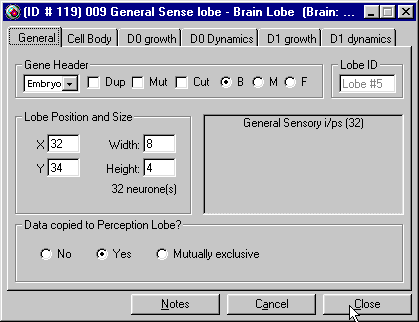
\epsfig {file=img/perception_gensense.png,width=7.39cm}} % 14.78cm
% 	\caption{Interface for Perception Lobe Design -- \textit{copying data} }
% 	\label{fig:perception_gensense}
% \end{figure}
% As can been seen from the above dialog box from the general sense lobe the options for perception are:
% \begin{itemize}
% 	\item No
% 	\item Yes
% 	\item Mutually exclusive
% \end{itemize}~\\
% The brain lobes that are marked as 'Yes' or 'Mutually exclusive' in an original norn are:
% \begin{longtable}{|p{0.25\textwidth}|p{0.15\textwidth}|p{0.65\textwidth}|}
% 	\hline \rowcolor[gray]{0.50} \multicolumn{3}{|c|}{Copied Lobes in Perception} \\
% 	\hline \rowcolor[gray]{0.75} \textbf{Lobe} & \textbf{Size} & \textbf{Data copied to perception lobe?} \\ \hline
% 	\endfirsthead
% 	\hline \rowcolor[gray]{0.50} \multicolumn{3}{|c|}{Copied Lobes in Perception} \\
% 	\hline \rowcolor[gray]{0.75} \textbf{Lobe} & \textbf{Size} & \textbf{Data copied to perception lobe?} \\ \hline
% 	\endhead
% 	\hline 
% 	\endfoot
% 
% 	Drive lobe		&	16 &	Mutually exclusive \\ \hline
% 	Verb lobe		&	16 &	Mutually exclusive \\ \hline
% 	General sense lobe	&	32 &	Yes \\ \hline
% 	Attention lobe 		&	40 &	Yes \\ \hline
% 
% 		\hline
% 	\caption{Copied Lobes in Perception}
% 	\label{tab:Copied_Lobes_in_Perception}\\
% \end{longtable}
% The perception lobe must have a number of cells equal to or greater than the total number of cells in all lobes marked as 'Yes' or 'Mutually exclusive'. The total number of cells in the above lobes equals 104. The size of the perception lobe is 112 so there is a little room to spare there.~\\
% My theory from observation is that starting from the lowest numbered perceptible lobe, the output of each cell of that lobe is copied to the lowest available cell in the perception lobe. So with the perceptible lobes listed above I think the mapping to the perception lobe cells will be:~\\~\\
% \begin{longtable}{|p{0.20\textwidth}|p{0.50\textwidth}|}
% 	\hline \rowcolor[gray]{0.50} \multicolumn{2}{|c|}{Mapping in Perception Lobe Cells} \\
% 	\hline \rowcolor[gray]{0.75} \textbf{Perception cell number} & \textbf{Other lobe cell number} \\ \hline
% 	\endfirsthead
% 	\hline \rowcolor[gray]{0.50} \multicolumn{2}{|c|}{Mapping in Perception Lobe Cells} \\
% 	\hline \rowcolor[gray]{0.75} \textbf{Perception cell number} & \textbf{Other lobe cell number} \\ \hline
% 	\endhead
% 	\hline 
% 	\endfoot
%  	
% 	0--15	&	Drive lobe 0-15 \\ \hline
% 	16--31	&	Verb lobe 0-15 \\ \hline
% 	32--63	&	General sense lobe 0-31 \\ \hline
% 	64--103	&	Attention lobe 0-39 \\ \hline
% 
% 		\hline
% 	\caption{Mapping in Perception Lobe Cells}
% 	\label{tab:Mapping_Perception_Lobe_Cells}\\
% \end{longtable}
% 
% I do not know what the setting 'Mutually exclusive' means. From my tests it appears to do the same as 'Yes' but further experimentation may show otherwise. The following examples will attempt to demonstrate whether my theory about how the perception lobe works and is mapped is correct or not.~\\
% For this example we start with a norn with the normal nine lobes selected in Creatures and we will test the lobes with Perceptible marked as 'Yes'. Run the BrainCellMonitor program, connect to Creatures, and use the 'Add' button to view the following Lobe/Cell/Dendrites:
% \begin{itemize}
% 	\item Lobe 0 Cell 32 Dendrite 0
% 	\item Lobe 0 Cell 63 Dendrite 0
% 	\item Lobe 5 Cell 0 Dendrite 0
% 	\item Lobe 5 Cell 31 Dendrite 0
% \end{itemize}
% 
% \begin{minipage}{0.4\linewidth}
% \begin{figure}[H]
% 	\centerline {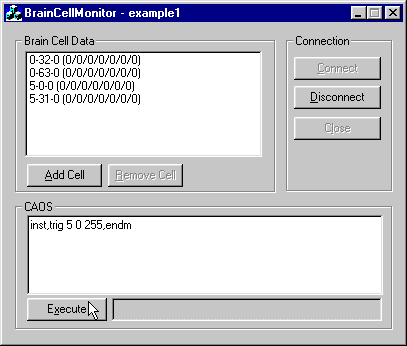
\epsfig {file=img/perception_example1.png,width=5cm}} % 14.36cm
% 	\caption{Interface for Perception Lobe Design -- \textit{how to complete data (1)} }
% 	\label{fig:perception_example1}
% \end{figure}
% \end{minipage}
% \begin{minipage}{0.1\linewidth}\end{minipage}
% \begin{minipage}{0.5\linewidth}
% This will allow us to view the first and last cell in the general sense lobe and compare it against the perceptible cell we think they will be copied to. We will now use CAOS commands to fire particular cells in the general sense lobe (lobe 5) and see if the corresponding cell in the perception lobe (lobe 0) fires with equivalent values.
% \end{minipage}~\\~\\
% 
% Try executing the CAOS command: $inst,trig 5 0 255,endm$. Notice how the perception lobe cell number 32 output number increases and starts to decrease in a similar way to the general sense lobe cell we just fired:
% \begin{figure}[H]
% 	\centerline {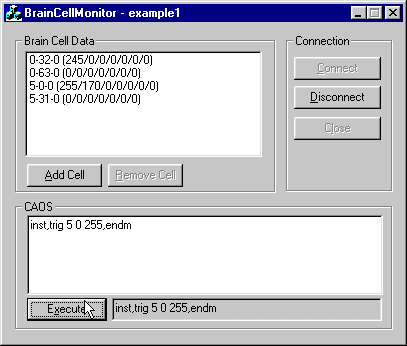
\epsfig {file=img/perception_example2.png,width=7.18cm}} % 14.36cm
% 	\caption{Interface for Perception Lobe Design -- \textit{how to complete data (2)} }
% 	\label{fig:perception_example2}
% \end{figure}
% 
% This seems to imply that our assumed mapping may be correct.~\\
% 
% Try executing the CAOS command: $inst,trig 5 31 255,endm$. Notice how the perception lobe cell number 63output number increases and starts to decrease in a similar way to the general sense lobe cell we just fired. This also seems to confirm our mapping. Try using different cell numbers with lobe 5 and you will see that the mapping we came up with is correct. Now we'll try it with the Attention lobe. Use BrainCellMonitor to view the following cells:
% \begin{itemize}
% 	\item Lobe 0 Cell 64 Dendrite 0
% 	\item Lobe 0 Cell 103 Dendrite 0
% 	\item Lobe 7 Cell 0 Dendrite 0
% 	\item Lobe 7 Cell 39 Dendrite 0
% \end{itemize}
% 
% Try executing the CAOS command: $inst,trig 7 0 255,endm$ and executing the CAOS command: $inst,trig 7 39 255,endm$. Once again you should see the equivalent perception lobes firing.~\\
% 
% You may notice that when doing the General sense example that if you fire both general sense lobes then both perception lobes also fire. But in the Attention example, firing both will only cause one perception lobe cell to fire - why is this? It is because the Attention lobe is marked 'Winner takes all'. This means that only the cell with the highest output actually fires - all the others get automatically set to zero and this data is copied to the perception lobe.~\\
% 
% Well what about the 'Mutually Exclusive' option? Lets try some examples with the Verb lobe which is marked "mutually exclusive". I don't use the Drive lobe just yet as the drives for a norn are constantly changing and can get in the way of our observations. Try viewing the following:
% \begin{itemize}
% 	\item Lobe 0 Cell 16 Dendrite 0
% 	\item Lobe 0 Cell 31 Dendrite 0
% 	\item Lobe 3 Cell 0 Dendrite 0
% 	\item Lobe 3 Cell 15 Dendrite 0
% \end{itemize}~\\
% Try executing the CAOS command: $inst,trig 3 0 255,endm$ and executing the CAOS command: $inst,trig 3 15 255,endm$. Once again you should see the equivalent perception lobes firing. The verb lobe is also marked 'Winner takes all' so you'll see similar effects to that shown in the Attention lobe. You can try examples with the drive lobe as well but as mentioned before the norn drives can get in the way of observation. ~\\
% The Mutually Exclusive option works in the same manner as lobes marked as 'Yes'. The difference between the two options appears when dendrites are linked between the perception lobe and the concept lobe. Usually from 1 to 3 perception cells are linked to a particular concept cell. The perception cells that are linked can change during the lifetime of a norn based on experiences it has encountered. But only one cell from a given Mutually Exclusive lobe can contribute to the forming of a particular concept. Drive is mutually exclusive so we can have a concept of 'hungry' but not 'hungry' and 'tired'. Verb lobe is also mutually exclusive so we can have a concept of being told to 'push' but not being told to 'push' and 'pull'.~\\
% I hope this tutorial/discussion was useful to you in examining the Perception lobe. If you come up with any interesting information I'd love to hear from you. I've updated the BrainActivity program to display the cell details in the perception lobe based on the above observations (as of version 1.3).~\\
% If you've been following this please send feedback to Chris Double (chris@double.co.nz) and let me know what you'd like to see. Thanks!~\\

% \section{CDR -- Dendrite Tutorial}
% $<$\textit{http://www.double.co.nz/creatures/tutorial3/tutorial3.htm}$>$~\\
% This tutorial introduces dendrites. It describes what they are and what can be done with them. All the information in this tutorial was discovered using experiments so it may not be completely correct. The information is pretty much a 'brain dump' of what I've encountered while playing around with brain lobes so it may not be organised particularly well. Any corrections, additions or comments are welcome.~\\

\clearpage

%% \section*{Section\markboth{Section}{Section}}
%% \addcontentsline{toc}{section}{Section}
%% \clearpage

%% \section*{Bibliography\markboth{Bibliography}{Bibliography}}
%% \addcontentsline{toc}{section}{Bibliography}
%% \bibliography{bibliography} %% .bib
%% \bibliographystyle{frplain} % plain or frplain

\end{document}
